\chapter{Resultados Experimentais}\label{cap:results}

\section{Aquisição de dados}

Para os experimentos realizados neste trabalho foi capturado um conjunto de vídeos no estacionamento do pavilhão João Calmon na Universidade de Brasília. Foram feitas duas seções de filmagens contínua, aonde três veículos se deslocavam pelo estacionamento e ocupavam vagas escolhidas arbitrariamente. O primeiro vídeo capturado foi utilizado para o treinamento da rede. O segundo vídeo foi dividido em oito vídeos de menor duração sobre os quais foram realizados os testes.

As filmagens foram realizadas por um drone modelo ????\ref{fig:???}. O drone foi controlado para que pairasse no ar em uma altura semelhante a de um poste de luz, a fim de capturar imagens de forma mais próxima possível de uma câmera de vídeo instalada em um poste de luz.

%Descobrir o modelo do drone e colocar uma imagem%

Para a aquisição das imagens utilizadas para o treinamento da rede, o primeiro vídeo passou por um processo semelhante ao processo de calibração do programa final descrito no capítulo \ref{cap:solucao}. Duas áreas de interesse foram determinadas de forma idêntica ao processo de escolha de ROIs do programa. Em seguida cada ROI foi dividida em trinta seções verticais. Três quadros do vídeo foram escolhidos de forma aleatória. As imagens correspondentes a cada seção de cada quadro escolhido foram extraídas em arquivos separados. Dessa maneira, as imagens utilizadas para o treinamento da rede neural foram construídas da mesma maneira que as imagens que seriam alimentadas a ela para classificação no futuro.

\section{Treinamento da rede neural artificial}

Uma vez adquiridas as imagens a serem utilizadas para o treinamento, cada uma delas foi separada manualmente em uma das duas categorias:veículo ou vaga vazia. Ao todo foram utilizadas $57$ imagens classificadas como veículo(categoria 1) e $59$ imagens classificadas como vaga vazia(categoria 2) totalizando $116$ imagens. Foram extraídas as características de cada imagem da forma descrita na seção \ref{sec:extracao}. Os vetores $x_s$ obtidos foram então concatenados de forma a criar duas matrizes. A primeira de dimensões $6x57$ representava as \textit{features} das imagens de carros e a segunda de dimensões $6x59$ as características das imagens de vagas desocupadas.

\begin{figure}
\centering
\begin{subfigure}{.1\textwidth}
  \centering
  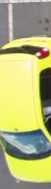
\includegraphics[width=.8\linewidth, height=5cm]{ocupada}
  \caption{}
  \label{fig:exemploRede:sub:ocupada}
\end{subfigure}%
\begin{subfigure}{.1\textwidth}
  \centering
  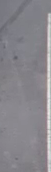
\includegraphics[width=.8\linewidth, height=5cm]{desocupada}
  \caption{}
  \label{fig:exemploRede:sub:desocupada}
\end{subfigure}
\centering
\caption{(a)Um exemplo de imagem classificada manualmente na classe 1.(b) Um exemplo de imagem classificada manualmente na classe 2.}
\label{fig:exemploRede}
\end{figure}

Para que pudesse ser feito o treinamento supervisionado da rede neural, duas matrizes de alvos foram construídas. Uma com dimensões $2x57$ e a outra com dimensões $2x59$. A primeira matriz com todas as colunas iguais a $\begin{psmallmatrix}1\\0\end{psmallmatrix}$ e a segunda com as colunas da forma $\begin{psmallmatrix}0\\1\end{psmallmatrix}$. Essas matrizes vão compor o gabarito utilizado para o treinamento supervisionado da rede.

As matrizes  de características de cada classe foram então concatenadas formando uma matriz de entrada $In_{6x116}$. O mesmo foi feito com as matrizes do gabarito, resultando na matriz $Target_{2x116}$. Em seguida as colunas dessas duas matrizes foram reorganizadas aleatoriamente, de forma que as mudanças feitas em $In$ fossem refletidas em $Out$, garantindo que não fosse perdida a relação entre as colunas de mesmo índice das matrizes. O resultado final deste processo é que cada coluna de $Target_{2x116}$ indica a classe da coluna correspondente de $In_{6x116}$.

Uma vez criadas essas duas matrizes, as entradas e seus respectivos alvos são separados em três conjuntos: o conjunto de treinamento, de validação e de testes. A divisão é feita de forma que $70\%$ das entradas são designadas ao conjunto de treinamento, $15\%$ designadas ao conjunto de validação e os $15\%$ restantes ao conjunto de testes. O conjunto de treinamento então é composto por duas matriz $Ti_{6x81}$ e $To_{2x81}$ que são iguais as primeira $81$ colunas de $In_{6x116}$ e $Target_{2x116}$ e representam os vetores descritores das entradas e seus gabaritos respectivamente. Os outros dois conjuntos são construídos de forma similar utilizando. O conjunto de validação é composto por matrizes de $18$ colunas e o de teste por matrizes de $17$ colunas.


A rede neural utilizada foi uma rede \textit{feed-forward} com três camadas. A camada oculta possui $15$ neurônios com função de ativação logística (\ref{eq:logistica}) e a camada de saída $2$ neurônios com função de ativação \textit{softmax} (\ref{eq:softmax}). A rede é submetida a um treinamento supervisionado com um limite de $1000$ iterações. Quando a situação de convergência é atingida, o treinamento para e o resultado é a rede final utilizada.


\section{Resultados Obtidos}

Para determinar a capacidade da programa de determinar se as seções verticais estão ocupadas ou livres, os resultados obtidos pelo programa foram comparados com os resultados que eram esperados de observadores humanos. Foram apresentados a três observadores, que chamaremos pelas iniciais F, M e P, um conjunto de oito vídeos que mostravam veículos estacionando ou saindo de vagas em um estacionamento descoberto. As áreas de interesse do vídeo foram definidas previamente e divididas em $30$ seções verticais. Dessa forma, todos os observadores e o programa analisaram seções verticais idênticas. 

Cada um dos observadores receberam as seguintes instruções:

\begin{itemize}
  \item As regiões de interesse e as seções são numeradas como indicado na figura \ref{instrucoes};
	\item Uma seção ocupada é aquela cuja maior parte de sua área está ocupada por um veículo;
	\item No momento inicial do vídeo ($0$ segundos), indique quais seções verticais estão ocupadas através do número das ROI e das seções, as outras serão assumidas como livres;
	\item Se a qualquer momento o estado de ocupação de uma seção mudar, indique o tempo da mudança, a seção onde ocorreu a mudança e a natureza da mudança(ocupada ou liberada).
\end{itemize}

\begin{figure}
\centering
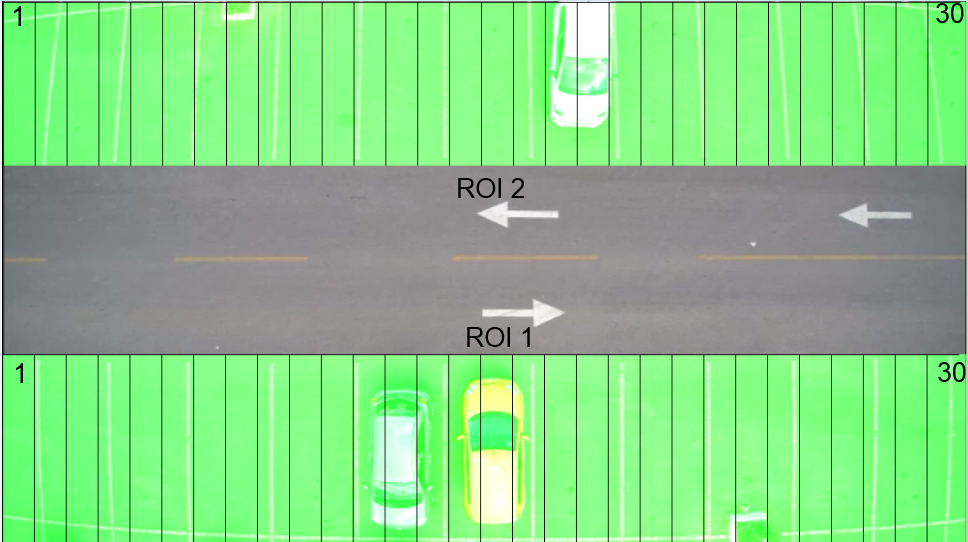
\includegraphics[width=8cm]{instrucoes}
\centering
\caption{Figura mostrando a divisão das ROIs e numeração das seções nos vídeos mostrados para os observadores humanos}
\label{fig:instrucao}
\end{figure}

Cada observador assistiu aos vídeos sozinho, sem interferência externa e sem conhecimento dos resultados do programa. De fato, a fim de evitar interferência, o programa só foi executado sobre os casos de teste após todos os observadores escolhidos terem entregado os resultados que obteram.

Para os testes apresentados a seguir, serão observadas somente aquelas seções que o programa ou os observadores determinaram como ocupadas. As demais seções serão consideradas livres. Chamaremos de um \textit{acerto} sempre que em um determinado segundo $t$, o programa e um observador concordam quanto a ocupação de uma seção vertical. Sendo assim, o programa pode atingir um máximo de $60$ acertos por segundo. A indicação da ocupação das seções pelos observadores não foi definida a cada segundo, mas considera-se que entre duas acusações de mudança de estado a ocupação das seções permanece a mesma. Sendo assim, podemos utilizar esses momentos para definir a ocupação em cada segundo do vídeo. Por exemplo, se um observador disser que a seção $10$ estava ocupada no momento inicial do vídeo e depois indicar que a mesma sessão foi liberada aos $8s$, a seção será considerada ocupada durante todos os momentos deste intervalo. 

Em seguida serão apresentados como um dos vídeos utilizados para os testes. Cada caso iniciará com uma breve descrição do movimento dos veículos no vídeo, a duração do vídeo e o número de acertos possíveis, seguidos de quatro tabelas, uma para cada observador e uma quarta para o programa. As tabelas indicam o tempo onde foram acusadas mudanças de estado nas seções. A primeira linha da tabela indica as seções ocupadas no momento inicial do vídeo e cada linha subsequente indica um momento em segundos quando houve mudança de estado de pelo menos uma seção e a ROI e número das seções. Finalmente, será calculada uma taxa de acerto que compara o desempenho do programa a cada observador e uma taxa final de acerto média para o caso de teste. A taxa de acerto para cada observador é calculada pela razão entre o número de acertos do programa e o número de acertos possíveis para o caso de teste e a taxa de acerto média é a média aritmética entre estes valores. Ao final destas seções uma breve análise dos resultados dos casos de teste será apresentada. Para que o leitor possa compara o desempenho do programa com suas próprias impressões, uma imagem dos momentos iniciais e finais de cada vídeo será mostrada junto de cada análise.


 
\subsection{Vídeo 1}

No primeiro caso de testes, o vídeo começa com um estacionamento vazio. Depois de alguns segundos um único veículo de cor branca entra na cena pela direita e estaciona em uma vaga na parte inferior da imagem. O vídeo tem $15s$ de duração, totalizando $900$ acertos possíveis.

\begin{figure}[!h]
\centering
\begin{subfigure}{.5\textwidth}
\centering
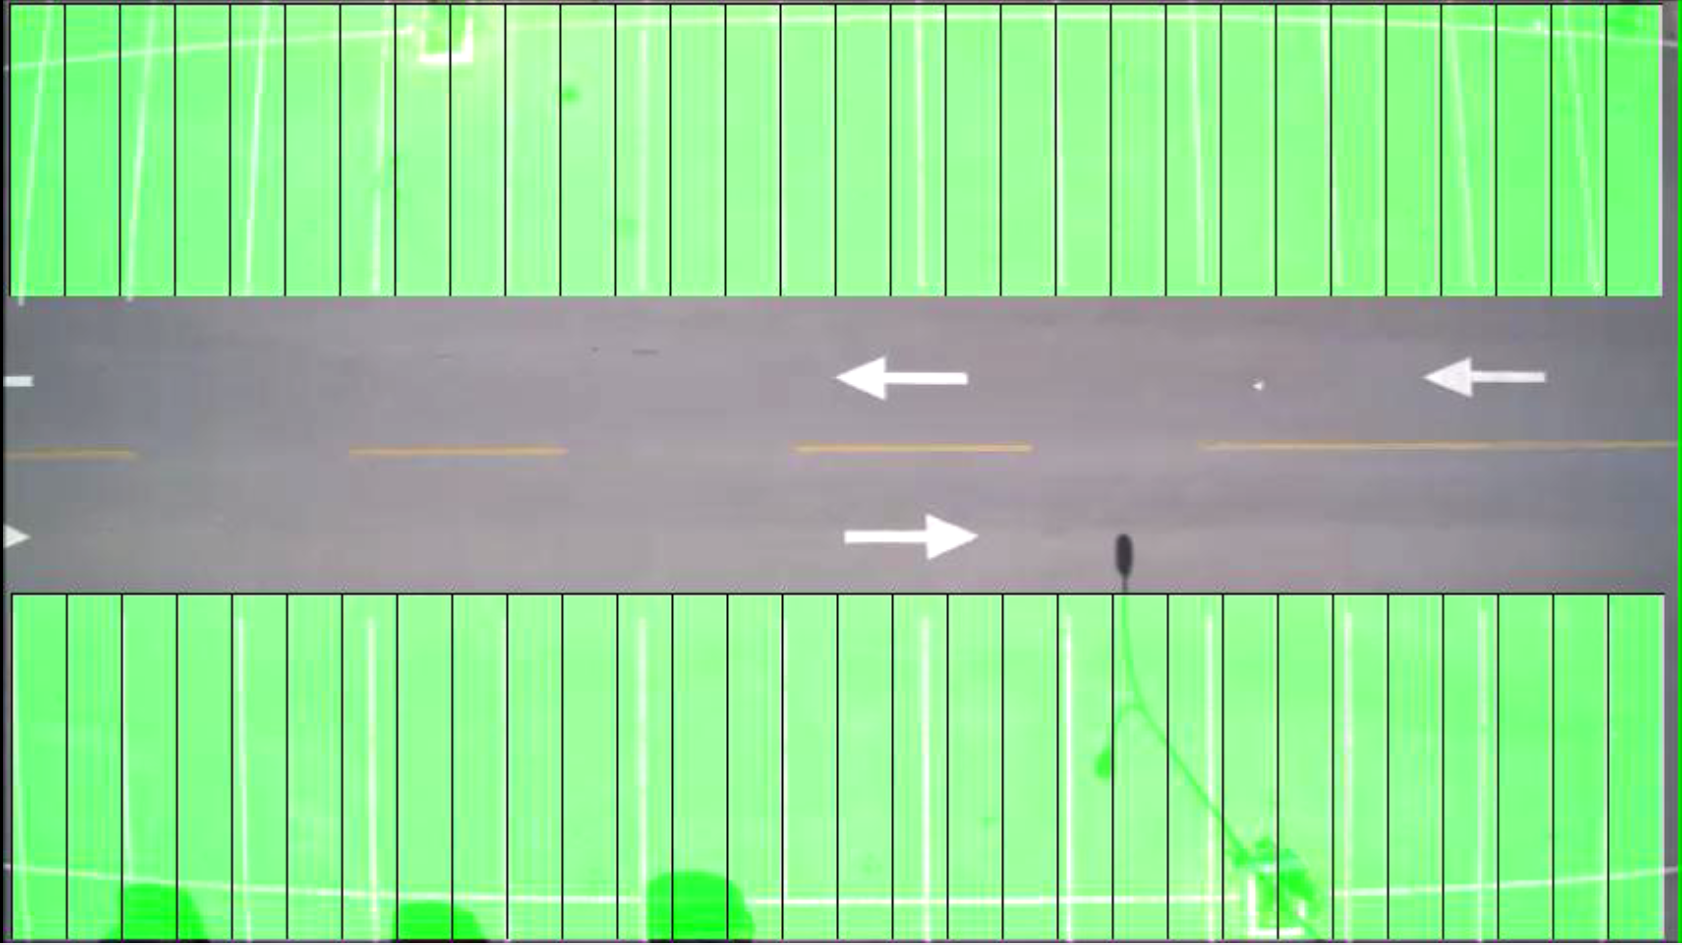
\includegraphics[width=.8\linewidth]{Video1Inicio}
\caption{}
\end{subfigure}\
\begin{subfigure}{.5\textwidth}
\centering
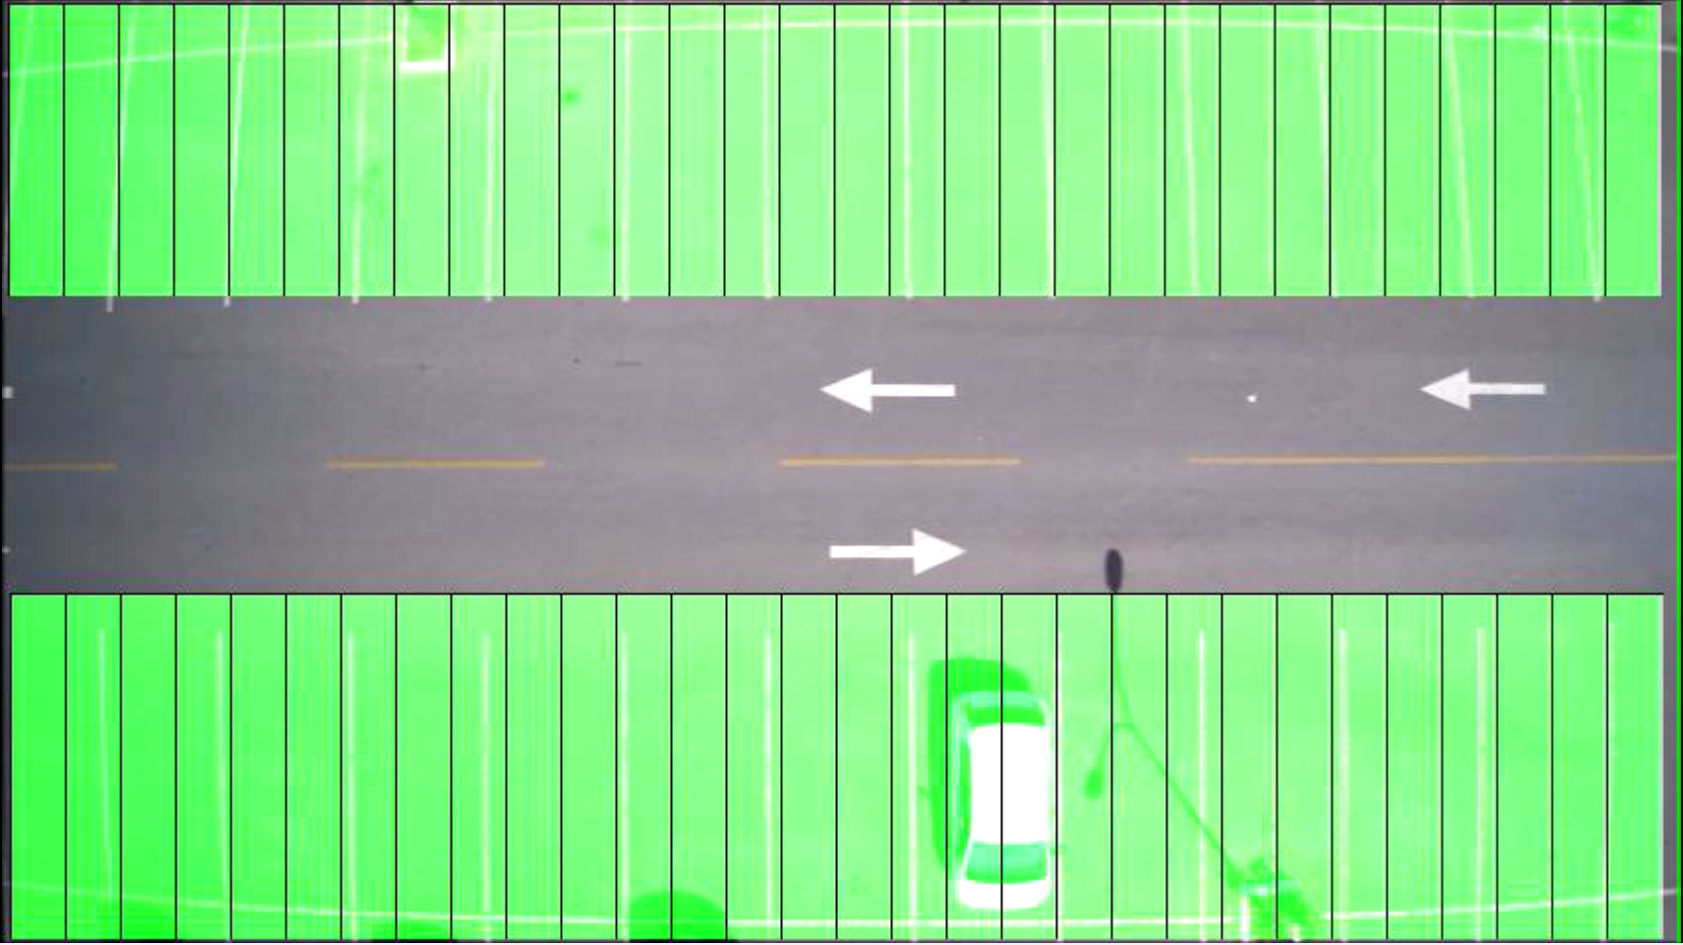
\includegraphics[width=.8\linewidth]{Video1Fim}
\caption{}
\end{subfigure}
\centering
\caption{(a) O momento inicial do vídeo 1. (b) O momento final do vídeo 1}%
\label{}%
\end{figure}


\begin{center}
\begin{tabular}{|c||c|}
\hline
\multicolumn{2}{|c|}{Observador F}  \\ \hline \hline
Tempo(s) & Acontecimento \\ \hline
0 & Nenhuma seção ocupada \\ \hline
10 & ROI 2: Seções 18 e 19 ocupadas. \\
\hline
\end{tabular}
\end{center}

\begin{center}
\begin{tabular}{|c||c|}
\hline
\multicolumn{2}{|c|}{Observador P}  \\ \hline \hline
Tempo(s) & Acontecimento \\ \hline
0 & Nenhuma seção ocupada \\ \hline
10 & ROI 2: Seções 18 e 19 ocupadas. \\
\hline
\end{tabular}
\end{center}

\begin{center}
\begin{tabular}{|c||c|}
\hline
\multicolumn{2}{|c|}{Observador M}  \\ \hline \hline
Tempo(s) & Acontecimento \\ \hline
0 & Nenhuma seção ocupada \\ \hline
9 & ROI 2: Seções 18 e 19 ocupadas. \\
\hline
\end{tabular}
\end{center}

\begin{center}
\begin{tabular}{|c||c|}
\hline
\multicolumn{2}{|c|}{Programa}  \\ \hline \hline
Tempo(s) & Acontecimento \\ \hline
0 & ROI 2:Seção 3 ocupada. \\ \hline
10 & ROI 2: Seções 18 e 19 ocupadas. \\ \hline
14 & ROI 2: Seção 3 liberada. \\
\hline
\end{tabular}
\end{center}

\begin{center}
\begin{tabular}{|c||c||c|}
\hline
Observador & Acertos & Taxa de acertos \\ \hline
F & 886 & 98,44\% \\  \hline
P & 886 & 98,44\% \\ \hline
M & 884 & 98,22\% \\ \hline
Média & 885,3 & 98,37\% \\
\hline
\end{tabular}
\end{center}

Neste caso de testes, o programa classifica errôneamente a seção $3$ da ROI $2$ durante quase toda a duração do vídeo. Apesar de persistente este erro tem pouca influência na indicação do número de vagas ocupadas, pois uma seção ocupada solitária não é suficiente para que o programa diminua o número de vagas livres.

Em relação ao observador M, o programa apresentou um atraso de $1s$ na classificação das seções $18$ e $19$ da ROI $2$, um atraso considerado aceitável, principalmente se considerarmos que o programa classificou estas mesmas seções no mesmo momento que os outros dois observadores.

\subsection{Vídeo 2}

Neste vídeo, um carro branco está estacionado no conjunto inferior de vagas. Um veículo cinza entra pela direita e estaciona no conjunto superior de vagas. O vídeo tem uma duração de $10s$, totalizando $600$ acertos possíveis.

\begin{figure}[!h]
\centering
\begin{subfigure}{.5\textwidth}
\centering
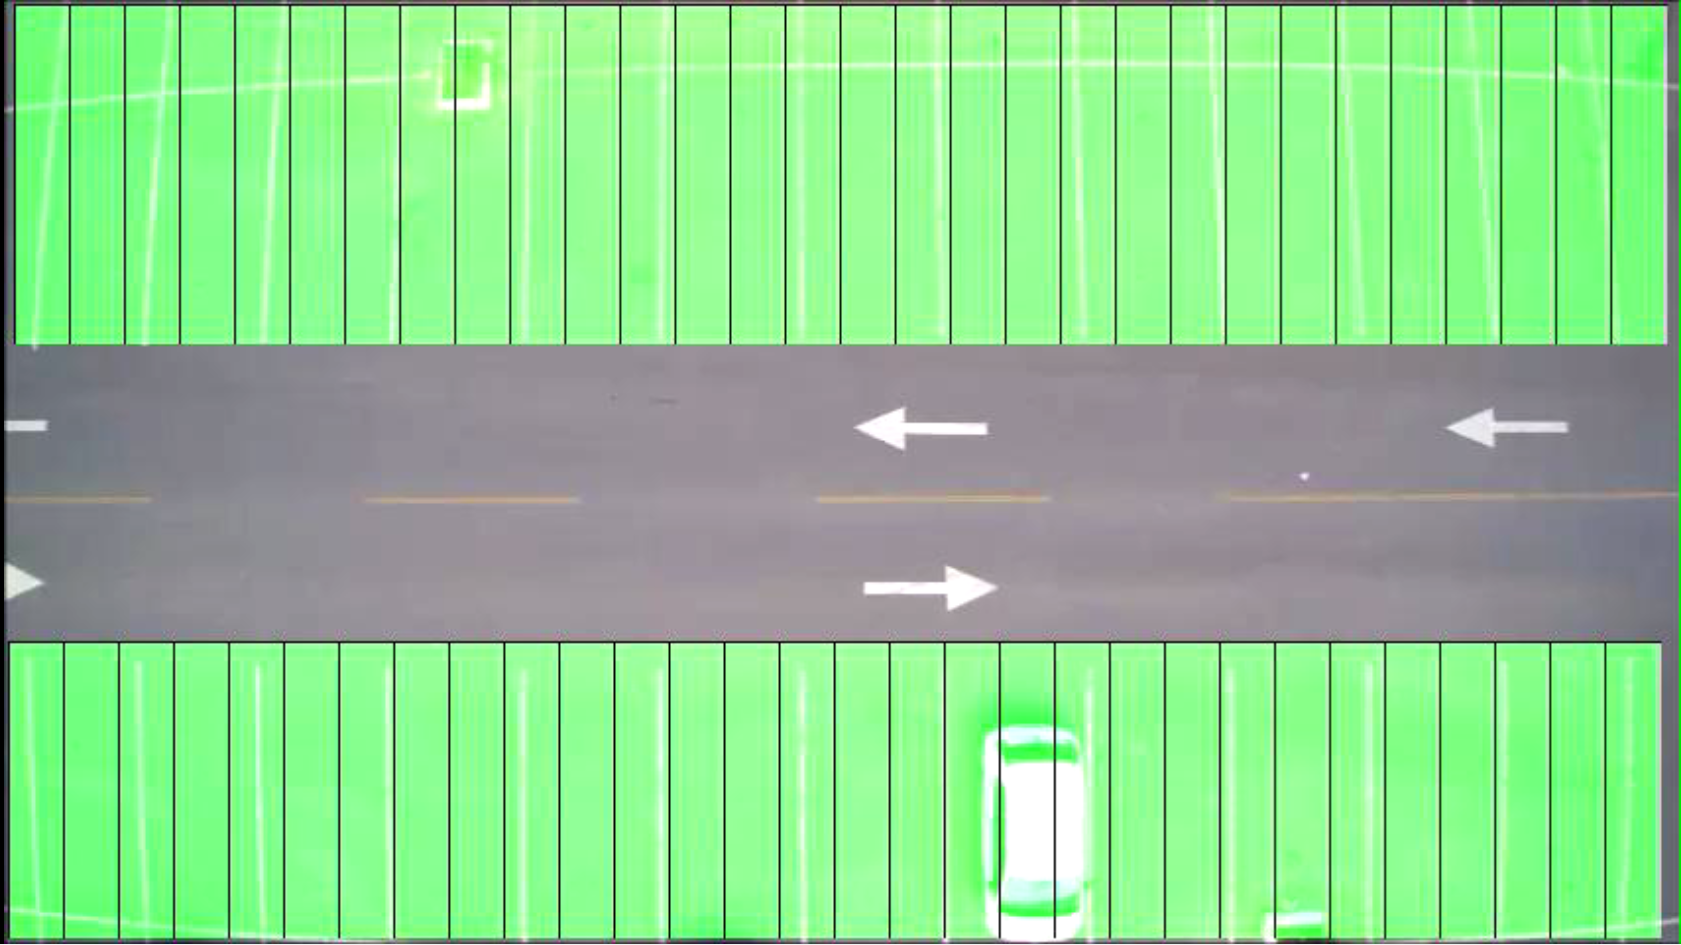
\includegraphics[width=.8\linewidth]{Video2Inicio}
\caption{}
\end{subfigure}\
\begin{subfigure}{.5\textwidth}
\centering
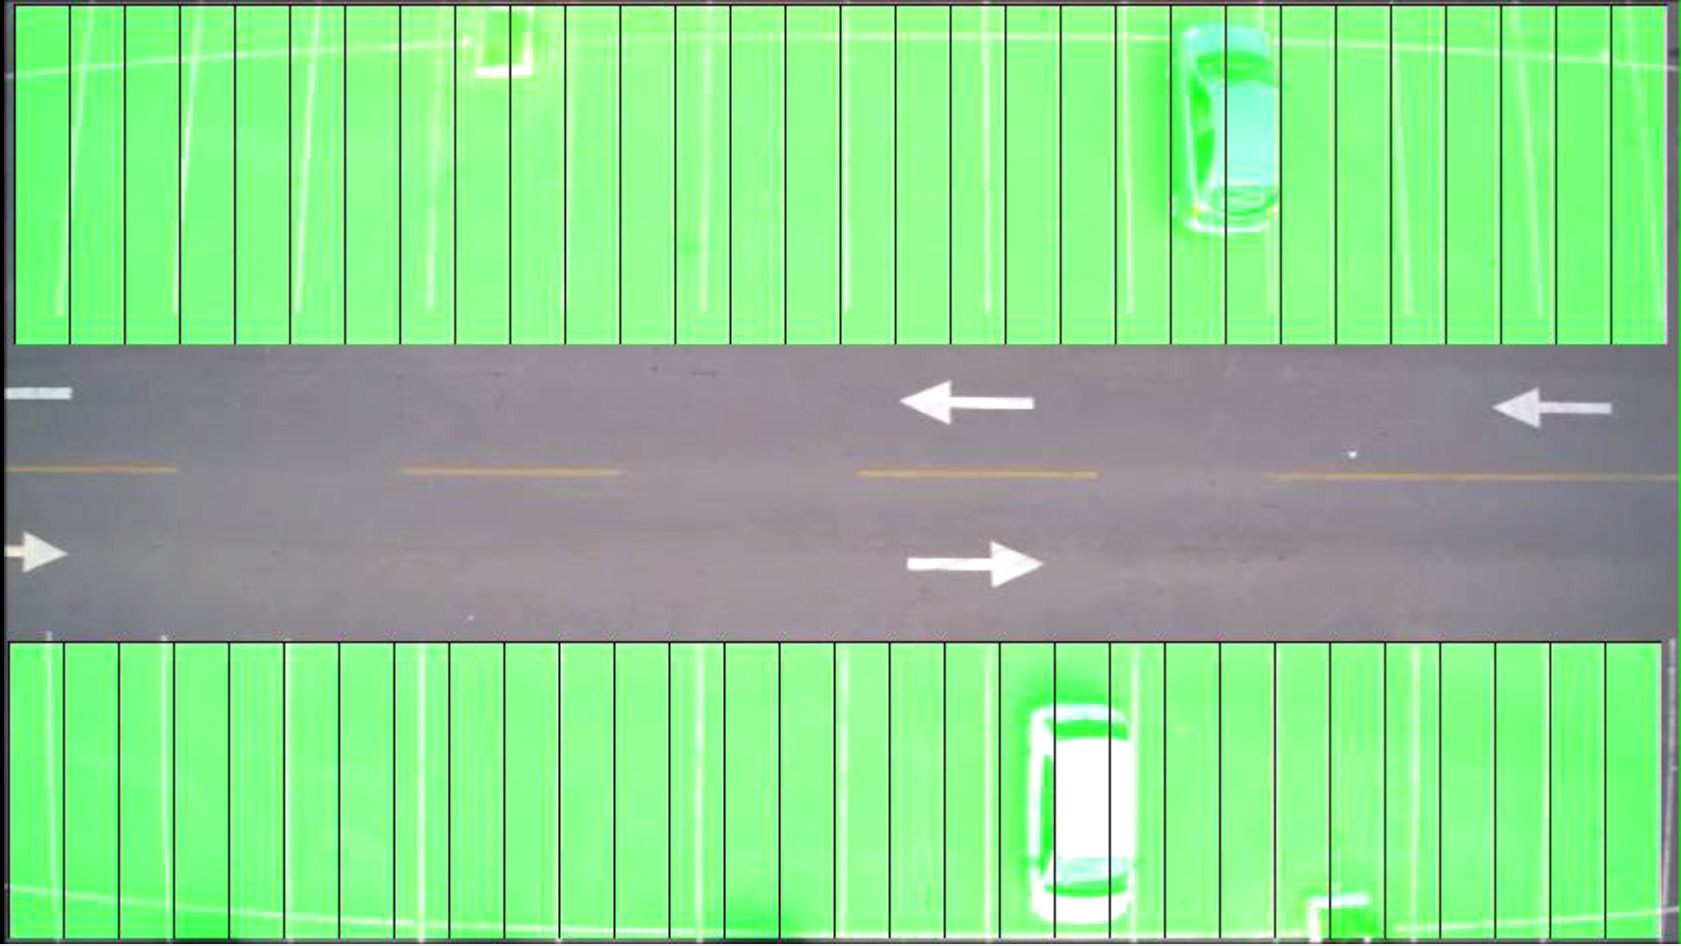
\includegraphics[width=.8\linewidth]{Video2Fim}
\caption{}
\end{subfigure}
\centering
\caption{(a) O momento inicial do vídeo 2. (b) O momento final do vídeo 2}%
\label{}%
\end{figure}


\begin{center}
\begin{tabular}{|c||c|}
\hline
\multicolumn{2}{|c|}{Observador F}  \\ \hline \hline
Tempo(s) & Acontecimento \\ \hline
0 & ROI 2: Seções 19 e 20 ocupadas \\ \hline
6 & ROI 1: Seções 21,22 e 23 ocupadas. \\
\hline
\end{tabular}
\end{center}

\begin{center}
\begin{tabular}{|c||c|}
\hline
\multicolumn{2}{|c|}{Observador P}  \\ \hline \hline
Tempo(s) & Acontecimento \\ \hline
0 & ROI 2: Seções 19 e 20 ocupadas \\ \hline
6 & ROI 1: Seções 20,21,22 ocupadas. \\
\hline
\end{tabular}
\end{center}

\begin{center}
\begin{tabular}{|c||c|}
\hline
\multicolumn{2}{|c|}{Observador M}  \\ \hline \hline
Tempo(s) & Acontecimento \\ \hline
0 & ROI 2: Seções 19 e 20 ocupadas \\ \hline
6 & ROI 1: Seções 21,22 e 23 ocupadas. \\
\hline
\end{tabular}
\end{center}

\begin{center}
\begin{tabular}{|c||c|}
\hline
\multicolumn{2}{|c|}{Programa}  \\ \hline \hline
Tempo(s) & Acontecimento \\ \hline
0 & ROI 2: Seções 18,19 e 20 ocupadas. \\ \hline
6 & ROI 1: Seções 21 e 22 ocupadas. \\ \hline
\hline
\end{tabular}
\end{center}

\begin{center}
\begin{tabular}{|c||c||c|}
\hline
Observador & Acertos & Taxa de acertos \\ \hline
F & 586 & 97,66\% \\  \hline
P & 586 & 97,66\% \\ \hline
M & 586 & 97,66\% \\ \hline
Média & 586 & 97,66\% \\
\hline
\end{tabular}
\end{center}

Neste caso de testes, houve discordância entre os observadores sobre as seções ocupadas pelo carro cinza na parte superior do vídeo. Porém o programa classificou como ocupadas as seções onde houve consenso entre os observadores.

O programa também classificou errôneamente a seção $18$ do ROI $2$ no momento inicial do vídeo. Novamente ele acerta nas seções onde há consenso entre os observadores. O erro é mais aceitável que o erro que ocorreu no vídeo $1$, por causa da proximidade da seção mal-classificada das seções onde houve acerto.

\subsection{Vídeo 3}

Neste vídeo, dois carros se encontram no estacionamento. Um veículo amarelo entra pela direita e estaciona na seção superior das vagas. O veículo branco sai pela parte de baixo da tela. Ele tem duração de $20s$ totalizando $1200$ acertos possíveis.

\begin{figure}[!h]
\centering
\begin{subfigure}{.5\textwidth}
\centering
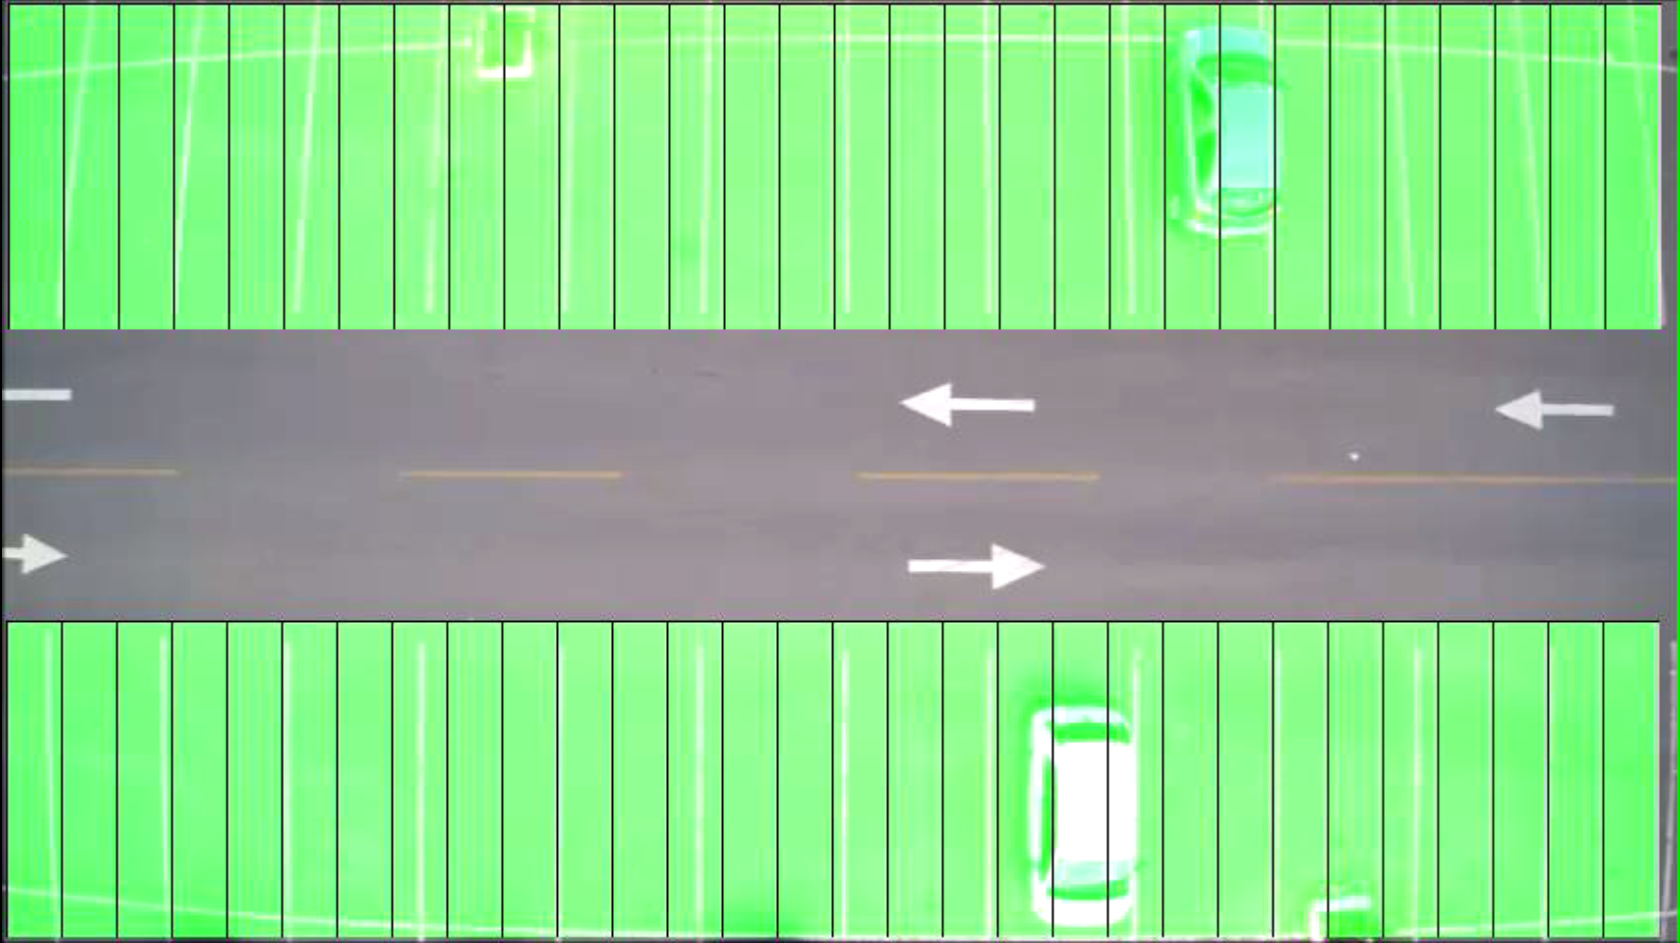
\includegraphics[width=.8\linewidth]{Video3Inicio}
\caption{}
\end{subfigure}\
\begin{subfigure}{.5\textwidth}
\centering
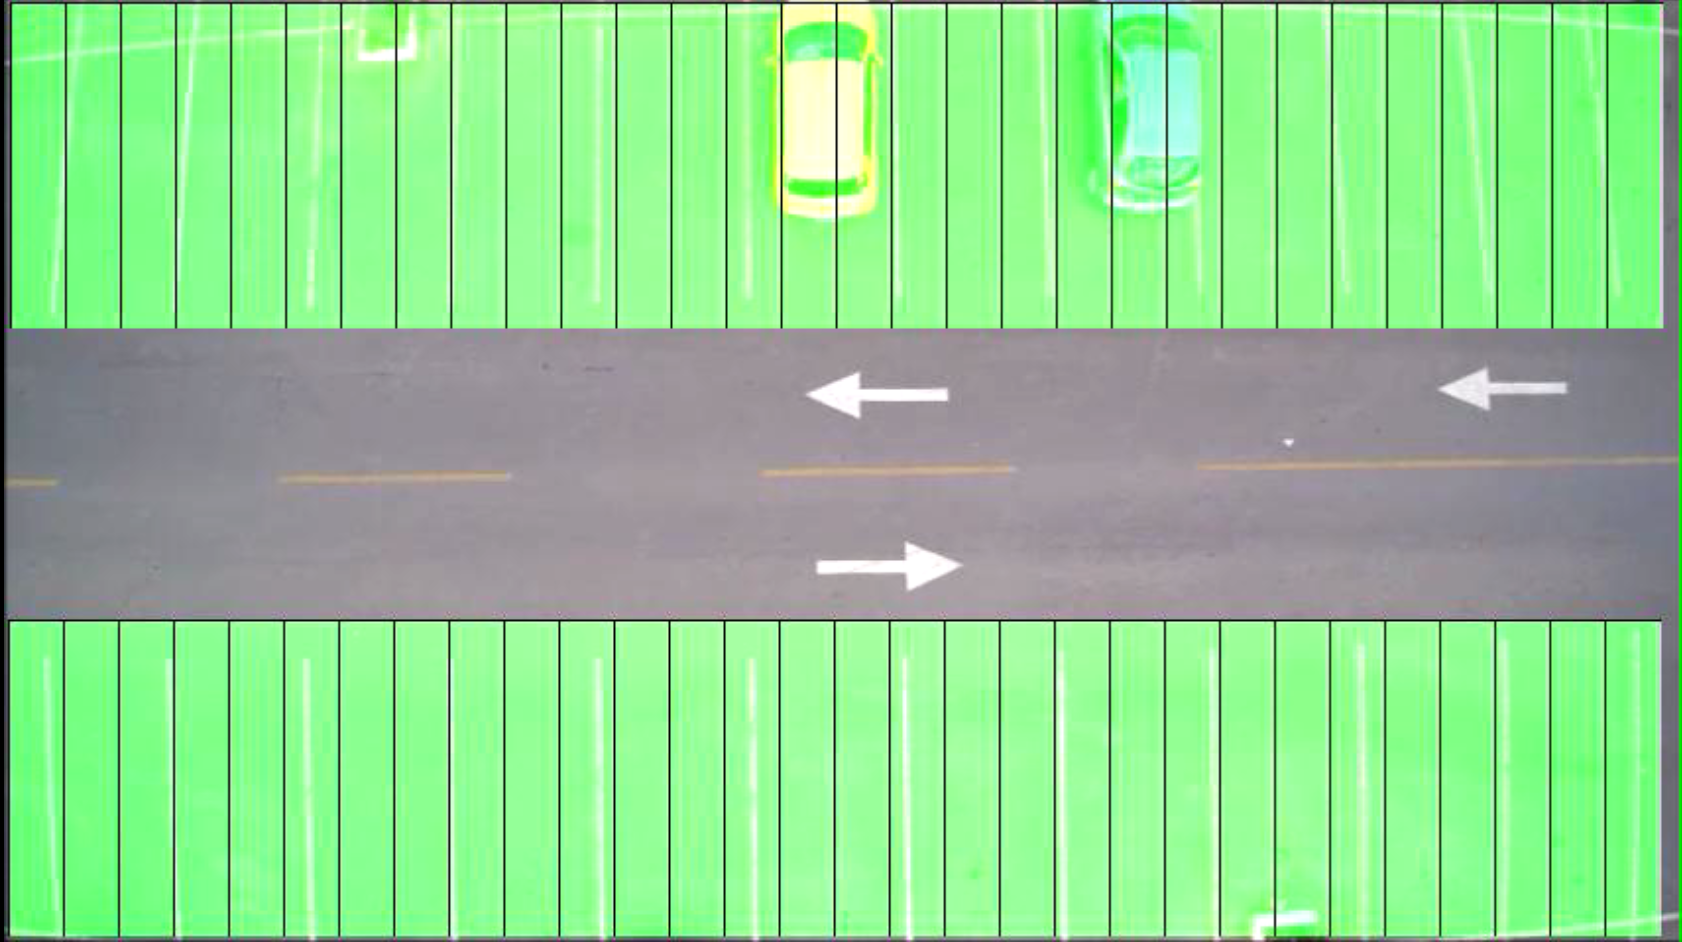
\includegraphics[width=.8\linewidth]{Video3Fim}
\caption{}
\end{subfigure}
\centering
\caption{(a) O momento inicial do vídeo 3. (b) O momento final do vídeo 3}%
\label{}%
\end{figure}

\begin{center}
\begin{tabular}{|c||c|}
\hline
\multicolumn{2}{|c|}{Observador F}  \\ \hline \hline
Tempo(s) & Acontecimento \\ \hline
0 & ROI 1: Seções 22 e 23 ocupadas. \\
 & ROI 2: 19,20 e 21 ocupadas \\ \hline
8 & ROI 1: Seções 16 e 17 ocupadas. \\ \hline
13 & ROI 2: Seções 18 e 19 liberadas. \\
\hline
\end{tabular}
\end{center}

\begin{center}
\begin{tabular}{|c||c|}
\hline
\multicolumn{2}{|c|}{Observador P}  \\ \hline \hline
Tempo(s) & Acontecimento \\ \hline
0 & ROI 1: Seções 22 e 23 ocupadas. \\
 & ROI 2: 20 e 21 ocupadas \\ \hline
9 & ROI 1: Seções 15,16 e 17 ocupadas. \\
\hline
\end{tabular}
\end{center}

\begin{center}
\begin{tabular}{|c||c|}
\hline
\multicolumn{2}{|c|}{Observador M}  \\ \hline \hline
Tempo(s) & Acontecimento \\ \hline
0 & ROI 1: Seções 22 e 23 ocupadas. \\
 & ROI 2: 20 e 21 ocupadas \\ \hline
8 & ROI 1: Seções 15,16 e 17 ocupadas. \\ \hline
14 & ROI 2: Seções 17,18 e 19 liberadas \\
\hline
\end{tabular}
\end{center}

\begin{center}
\begin{tabular}{|c||c|}
\hline
\multicolumn{2}{|c|}{Programa}  \\ \hline \hline
Tempo(s) & Acontecimento \\ \hline
0 & ROI 1: Seções 22 e 23 ocupadas. \\
 & ROI 2: 19,20 e 21 ocupadas \\ \hline
1 & ROI 1: Seção 23 liberada. \\ \hline
2 & ROI 1: Seção 23 ocupada. \\ \hline
4 & ROI 1: Seção 23 liberada. \\ \hline
8 & ROI 1: Seções 16 e 17 ocupadas. \\ \hline
9 & ROI 2: Seção 21 liberada. \\ 
 & ROI 2: Seções 18 e 24 ocupadas \\ \hline
11 & ROI 1: Seção 20 ocupada. \\ 
 & ROI 2: Seção 24 liberada. \\ \hline
13 & ROI 1: Seção 20 liberada. \\
 & ROI 2: Seção 18,19 e 20 liberada. \\ \hline
16 & ROI 1: Seção 20 ocupada. \\ \hline
19 & ROI 1: Seção 20 liberada. \\
\hline
\end{tabular}
\end{center}

\begin{center}
\begin{tabular}{|c||c||c|}
\hline
Observador & Acertos & Taxa de acertos \\ \hline
F & 1165 & 97,08\% \\  \hline
P & 1113 & 92,75\% \\ \hline
M & 1136 & 94,66\% \\ \hline
Média & 1138 & 94,83\% \\
\hline
\end{tabular}
\end{center}

Esse caso de teste possui alguns problemas causados principalmente por causa da movimentação do \textit{drone} no momento da gravação. Essa movimentação faz com que partes da imagem passem a ocupar seções diferentes, criando algumas incosistências. Repare que por volta dos $14s$ dois dos observadores disseram que a seção $18$ da ROI $2$ foi liberada, apesar de nunca terem acusado que ela estava ocupada anteriormente. Essa inconsistência ocorre porque entre o início do vídeo esse momento, o \textit{drone} utilizado para a gravação se movimenta e faz com que o veículo que estava ocupando as  seções $19$ e $20$ ocupe as seções $18$ e $19$. Esse problema acontece em outros casos de teste em menor proporção.

Apesar destes problemas, o teste sobre esse vídeo ainda possui resultados interessantes e úteis. Uma vantagem do uso de um sistema automatizado se mostra neste caso de teste. O observador \textit{P} não percebeu que um veículo saia da tela por volta dos $14$ segundos e por isso não acusou a mudança de estado de nenhuma seção nesse momento. Uma falha que não ocorre no programa. 

Através deste caso também percebe-se que o programa tem dificuldade em classificar corretamente as seções ocupadas pelo veículo cinza na ROI $1$, evidenciada principalmente pela flutuação da classificação das seções $23$ e $20$.



\subsection{Vídeo 4}

Neste vídeo, o veículo branco entra em cena pela parte superior da tela e estaciona entre os outros dois carros. O carro cinza sai da vaga que ocupava e estaciona em uma na área inferior. Duração de $30s$, portanto $1800$ possíveis acertos.

\begin{figure}[!h]
\centering
\begin{subfigure}{.5\textwidth}
\centering
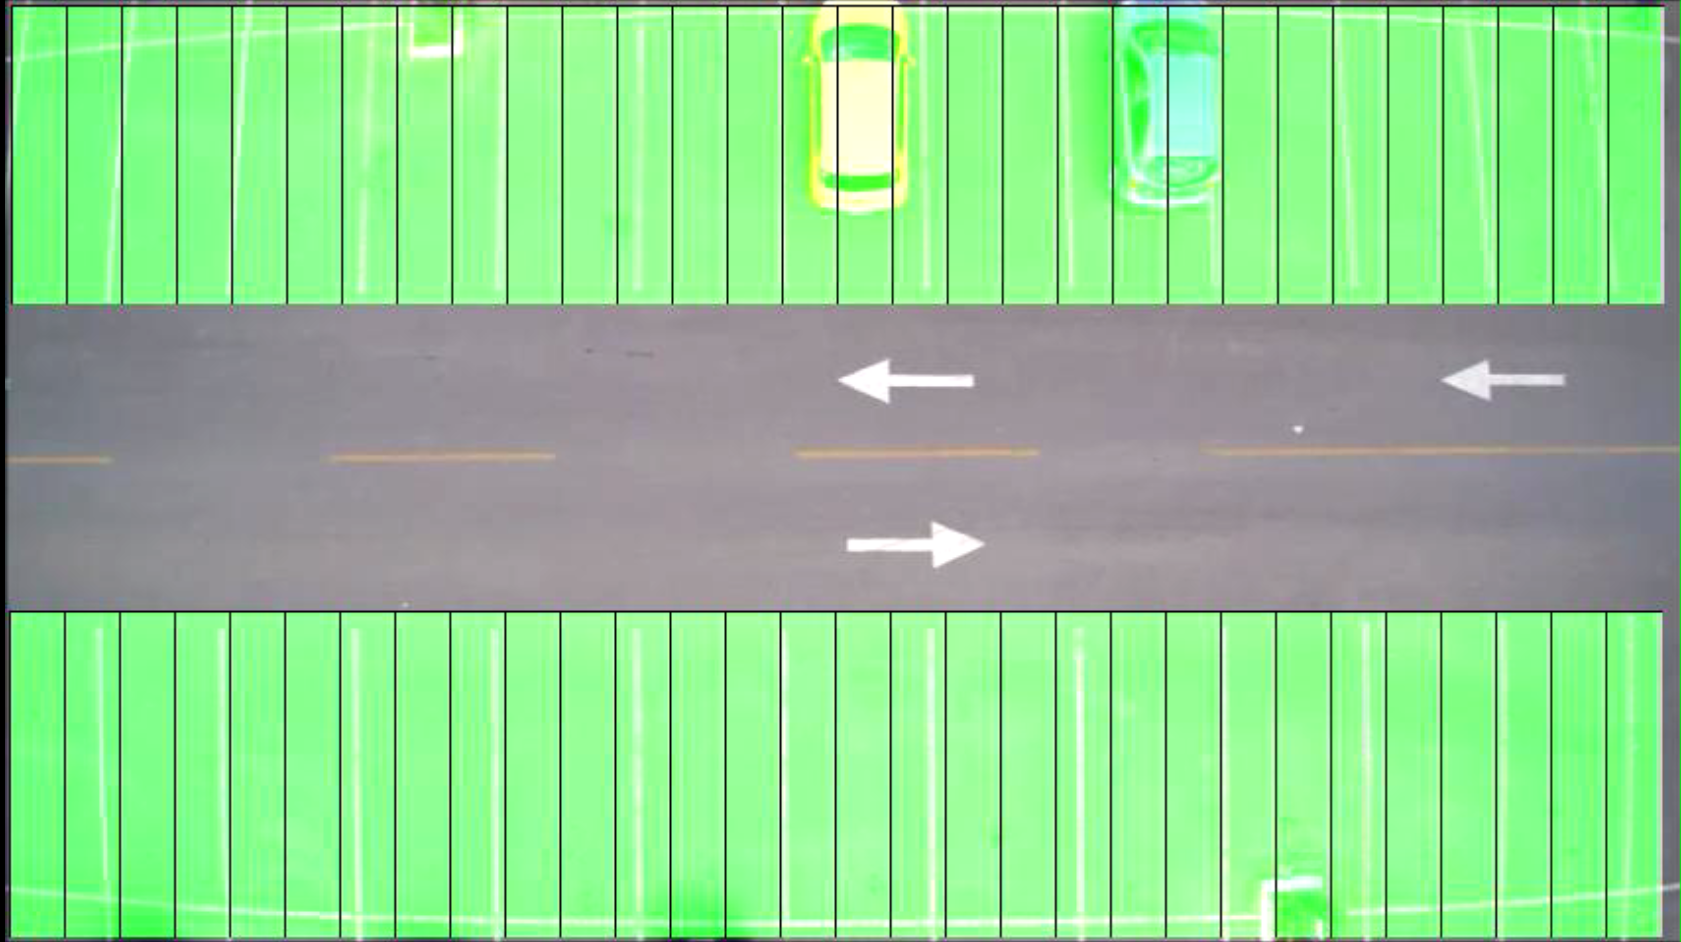
\includegraphics[width=.8\linewidth]{Video4Inicio}
\caption{}
\end{subfigure}\
\begin{subfigure}{.5\textwidth}
\centering
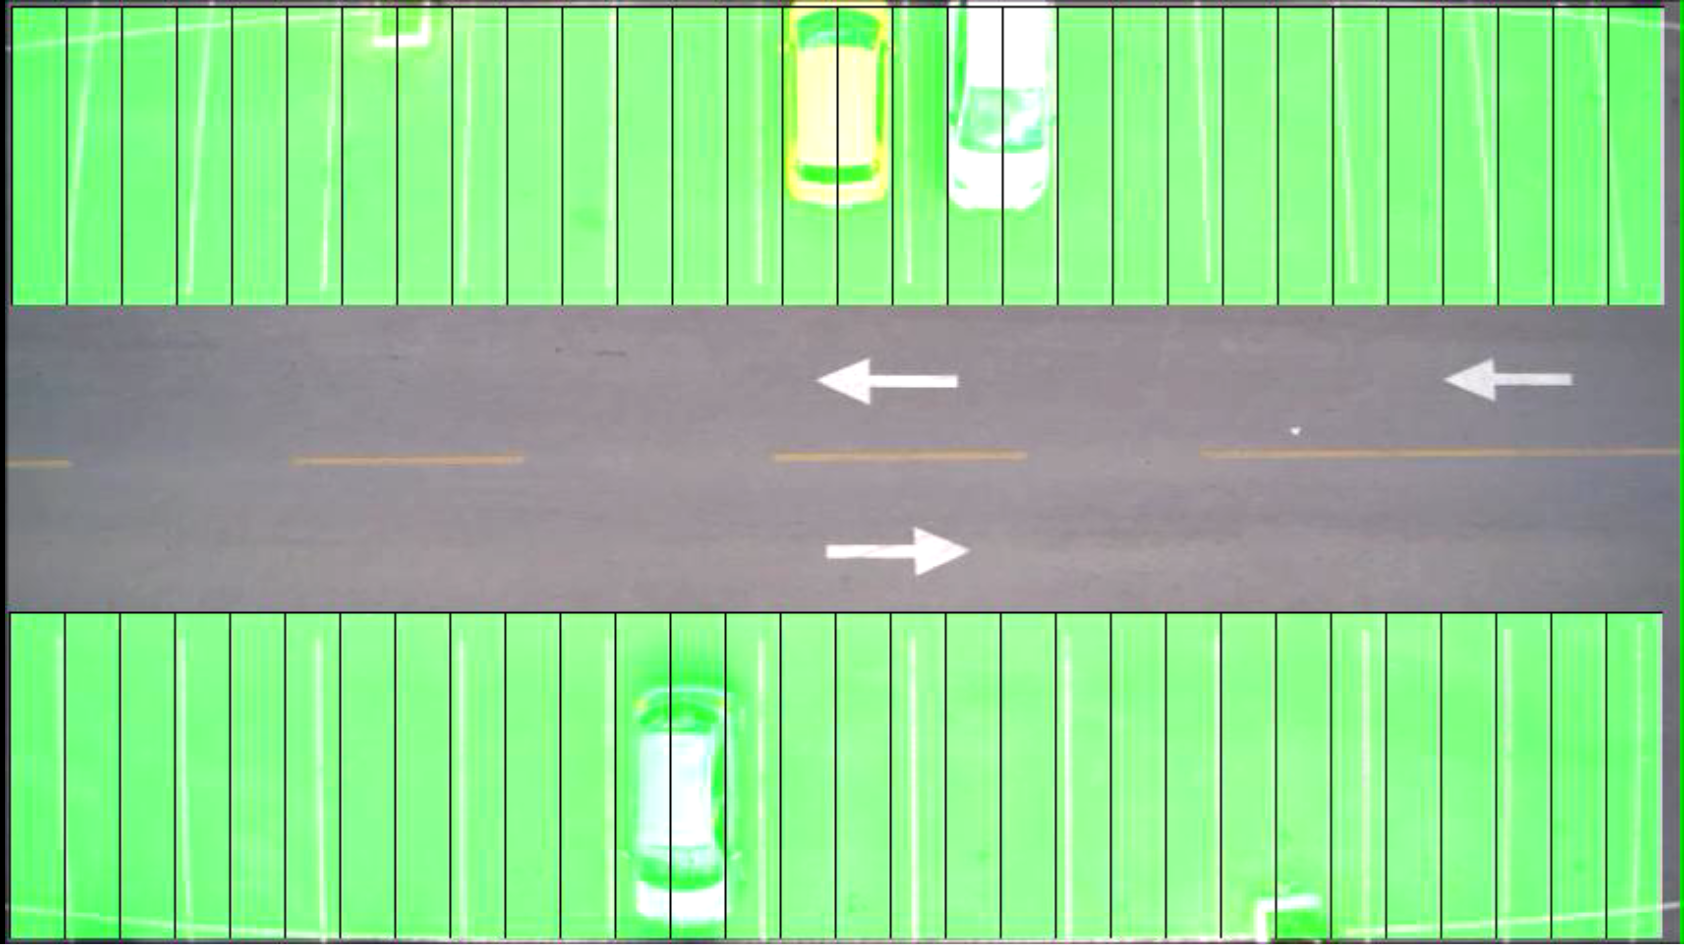
\includegraphics[width=.8\linewidth]{Video4Fim}
\caption{}
\end{subfigure}
\centering
\caption{(a) O momento inicial do vídeo 4. (b) O momento final do vídeo 4}%
\label{}%
\end{figure}

\begin{center}
\begin{tabular}{|c||c|}
\hline
\multicolumn{2}{|c|}{Observador F}  \\ \hline \hline
Tempo(s) & Acontecimento \\ \hline
0 & ROI 1: Seções 15,16,21 e 22 ocupadas. \\ \hline
7 & ROI 1: Seções 19 e 20 ocupadas. \\ \hline
16 & ROI 1: Seções 21 e 22 liberadas. \\ \hline
28 & ROI 2: Seções 12 e 13 ocupadas. \\
\hline
\end{tabular}
\end{center}

\begin{center}
\begin{tabular}{|c||c|}
\hline
\multicolumn{2}{|c|}{Observador P}  \\ \hline \hline
Tempo(s) & Acontecimento \\ \hline
0 & ROI 1: Seções 15,16,17,20 e 21 ocupadas. \\ \hline
8 & ROI 1: Seções 18 e 19 ocupadas. \\ \hline
18 & ROI 1: Seções 21 e 22 liberadas \\ \hline
29 & ROI 2: 12,13 e 14 ocupadas \\
\hline
\end{tabular}
\end{center}

\begin{center}
\begin{tabular}{|c||c|}
\hline
\multicolumn{2}{|c|}{Observador M}  \\ \hline \hline
Tempo(s) & Acontecimento \\ \hline
0 & ROI 1: Seções 15,16,20 e 21 ocupadas. \\ \hline
6 & ROI 1: Seções 18 e 19 ocupadas. \\ \hline
17 & ROI 1: Seções 21 e 22 liberadas \\ \hline
28 & ROI 2: Seções 12,13 e 14 ocupadas \\
\hline
\end{tabular}
\end{center}

\begin{center}
\begin{tabular}{|c||c|}
\hline
\multicolumn{2}{|c|}{Programa}  \\ \hline \hline
Tempo(s) & Acontecimento \\ \hline
0 & ROI 1: Seções 15,16,20 e 21 ocupadas. \\ \hline
6 & ROI 1: Seções 18 e 19 ocupadas. \\ \hline
11 & ROI 1: Seção 22 ocupada. \\ \hline
14 & ROI 1: Seção 22 liberada. \\ \hline
23 & ROI 1: Seção 20 liberada. \\ \hline
28 & ROI 2: Seções 12 e 13 ocupadas. \\
\hline
\end{tabular}
\end{center}

\begin{center}
\begin{tabular}{|c||c||c|}
\hline
Observador & Acertos & Taxa de acertos \\ \hline
F & 1750 & 97,22\% \\  \hline
P & 1749 & 97,16\% \\ \hline
M & 1772 & 98,44\% \\ \hline
Média & 1757 & 97,61\% \\
\hline
\end{tabular}
\end{center}

Este vídeo reforça a dificuldade do programa de classificar corretamente as seções ocupadas pelo veículo cinza. Porém a dificuldade parece não acontecer quando este carro estaciona na região inferior, quando o programa consegue que o veículo ocupa as mesmas seções que os observadores humanos.


\subsection{Vídeo 5}

Um veículo desocupa a sua vaga sainda pela parte superior da tela. Duração de $10s$ ou $600$ possíveis acertos.

\begin{figure}[!h]
\centering
\begin{subfigure}{.5\textwidth}
\centering
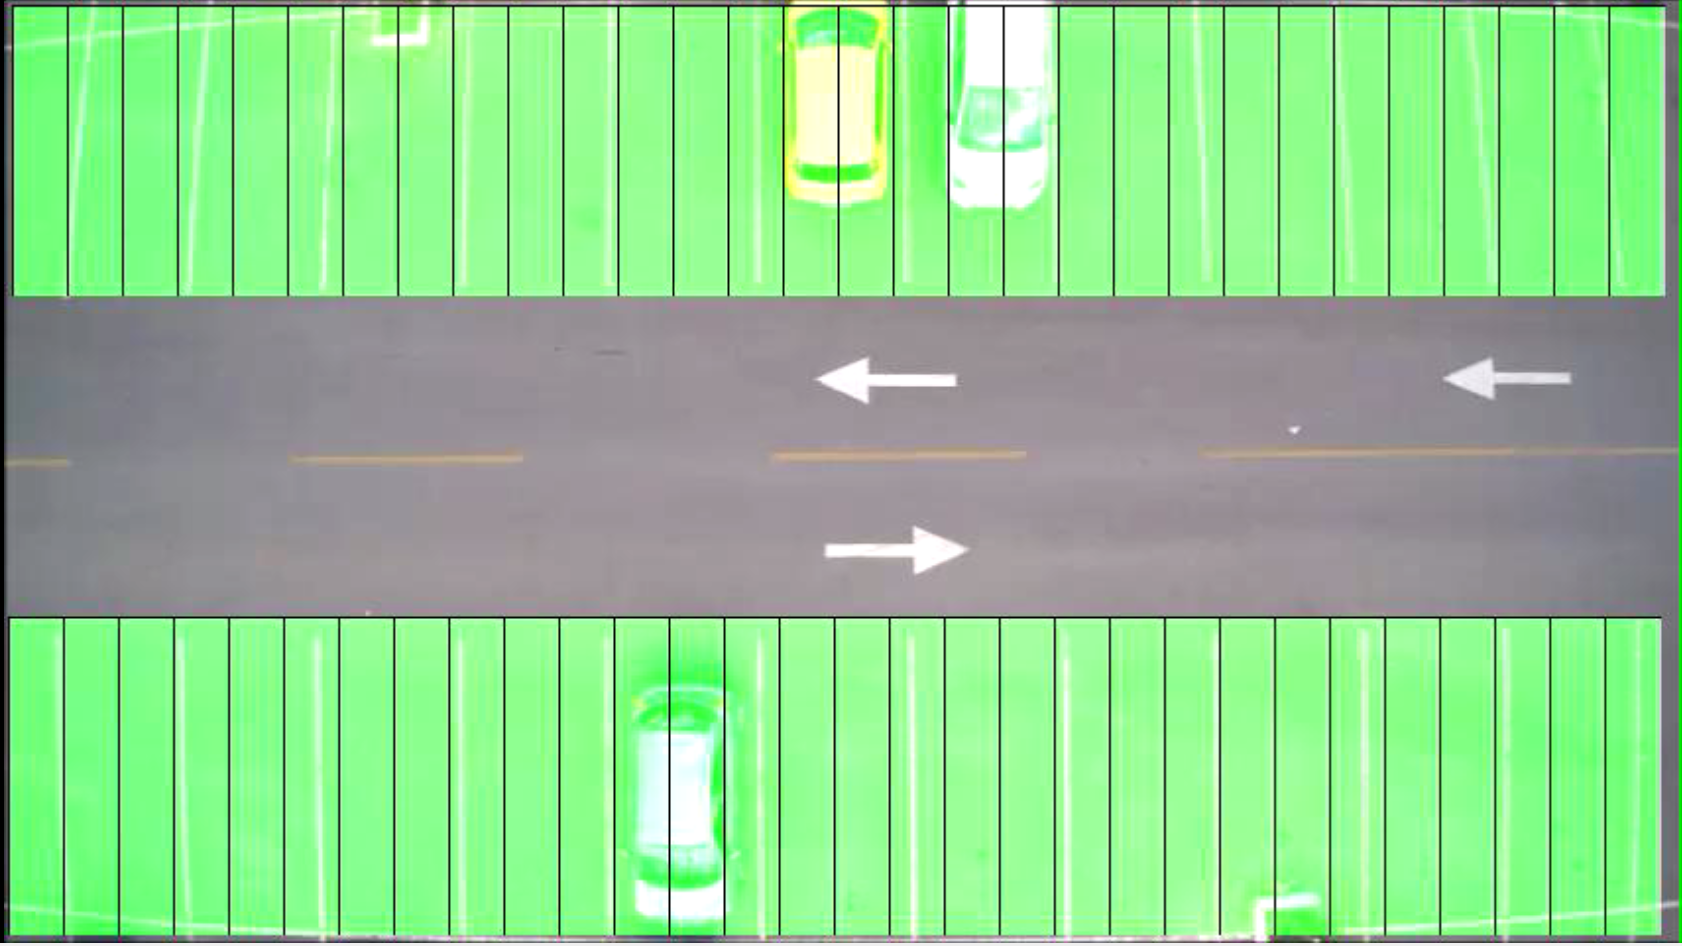
\includegraphics[width=.8\linewidth]{Video5Inicio}
\caption{}
\end{subfigure}\
\begin{subfigure}{.5\textwidth}
\centering
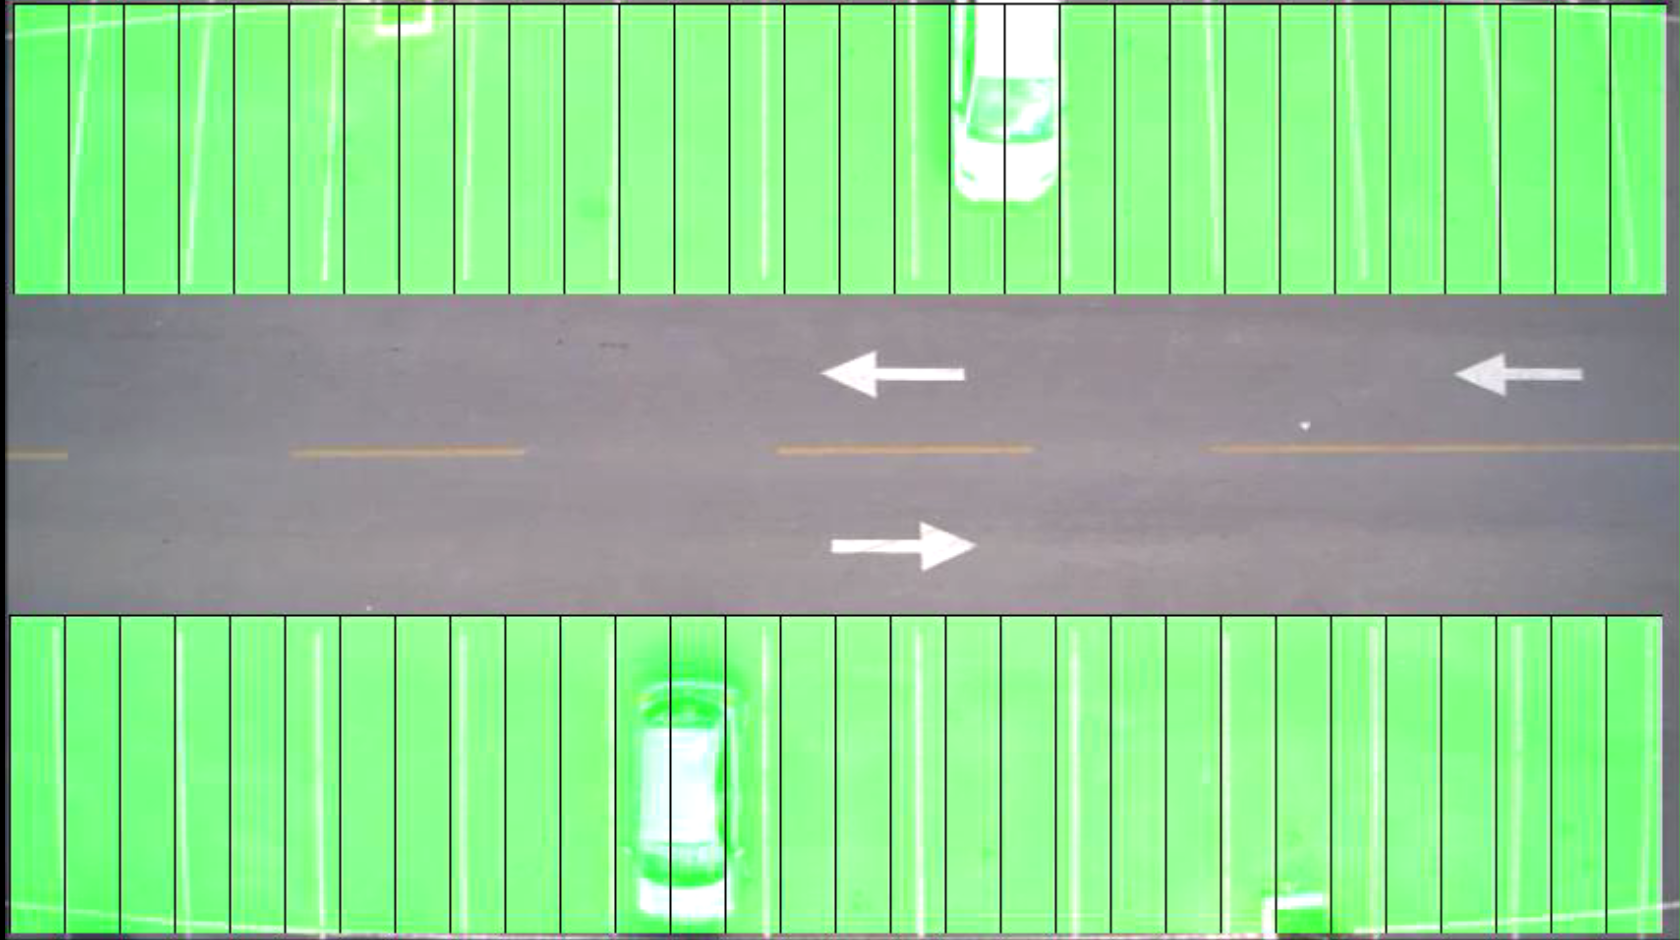
\includegraphics[width=.8\linewidth]{Video5Fim}
\caption{}
\end{subfigure}
\centering
\caption{(a) O momento inicial do vídeo 5. (b) O momento final do vídeo 5}%
\label{}%
\end{figure}

\begin{center}
\begin{tabular}{|c||c|}
\hline
\multicolumn{2}{|c|}{Observador F}  \\ \hline \hline
Tempo(s) & Acontecimento \\ \hline
0 & ROI 1: Seções 15,16,18 e 19 ocupadas. \\
 & ROI 2: Seções 12 e 13 ocupadas. \\ \hline
3 & ROI 1: Seções 15 e 16 liberadas. \\
\hline
\end{tabular}
\end{center}

\begin{center}
\begin{tabular}{|c||c|}
\hline
\multicolumn{2}{|c|}{Observador P}  \\ \hline \hline
Tempo(s) & Acontecimento \\ \hline
0 & ROI 1: Seções 15,16,18 e 19 ocupadas. \\
 & ROI 2: Seções 12,13 e 14 ocupadas. \\ \hline
4 & ROI 1: Seções 15 e 16 liberadas. \\
\hline
\end{tabular}
\end{center}

\begin{center}
\begin{tabular}{|c||c|}
\hline
\multicolumn{2}{|c|}{Observador M}  \\ \hline \hline
Tempo(s) & Acontecimento \\ \hline
0 & ROI 1: Seções 15,16,18 e 19 ocupadas. \\
 & ROI 2: Seções 12,13 e 14 ocupadas. \\ \hline
3 & ROI 1: Seções 15 e 16 liberadas. \\
\hline
\end{tabular}
\end{center}

\begin{center}
\begin{tabular}{|c||c|}
\hline
\multicolumn{2}{|c|}{Programa}  \\ \hline \hline
Tempo(s) & Acontecimento \\ \hline
0 & ROI 1: Seções 15,16,18 e 19 ocupadas. \\
 & ROI 2: Seções 12 e 13 ocupadas. \\ \hline
1 & ROI 1: Seção 17 ocupada. \\ \hline
3 & ROI 1: Seções 15 e 16 liberadas. \\ \hline
4 & ROI 1: Seção 17 liberada. \\
\hline
\end{tabular}
\end{center}

\begin{center}
\begin{tabular}{|c||c||c|}
\hline
Observador & Acertos & Taxa de acertos \\ \hline
F & 597 & 99,50\% \\  \hline
P & 585 & 97,50\% \\ \hline
M & 587 & 97,83\% \\ \hline
Média & 1757 & 97,61\% \\
\hline
\end{tabular}
\end{center}

Um caso de testes simples, onde os erros ocorreram principalmente por causa da natureza subjetiva do que configura uma seção ocupada. O programa classifica a seção $17$ como ocupada e os observadores não. Por outro lado, dois dos observadores acharam que a seção $14$ da ROI $2$ estava ocupada, descordando do programa.

\subsection{Vídeo 6}

Neste vídeo o veículo amarelo entra na cena pela parte inferior da tela. O veículo branco desocupa sua vaga e sai da tela pelo lado esquerdo. O vídeo tem $13s$ totalizando $780$ acertos possíveis.

\begin{figure}[!h]
\centering
\begin{subfigure}{.5\textwidth}
\centering
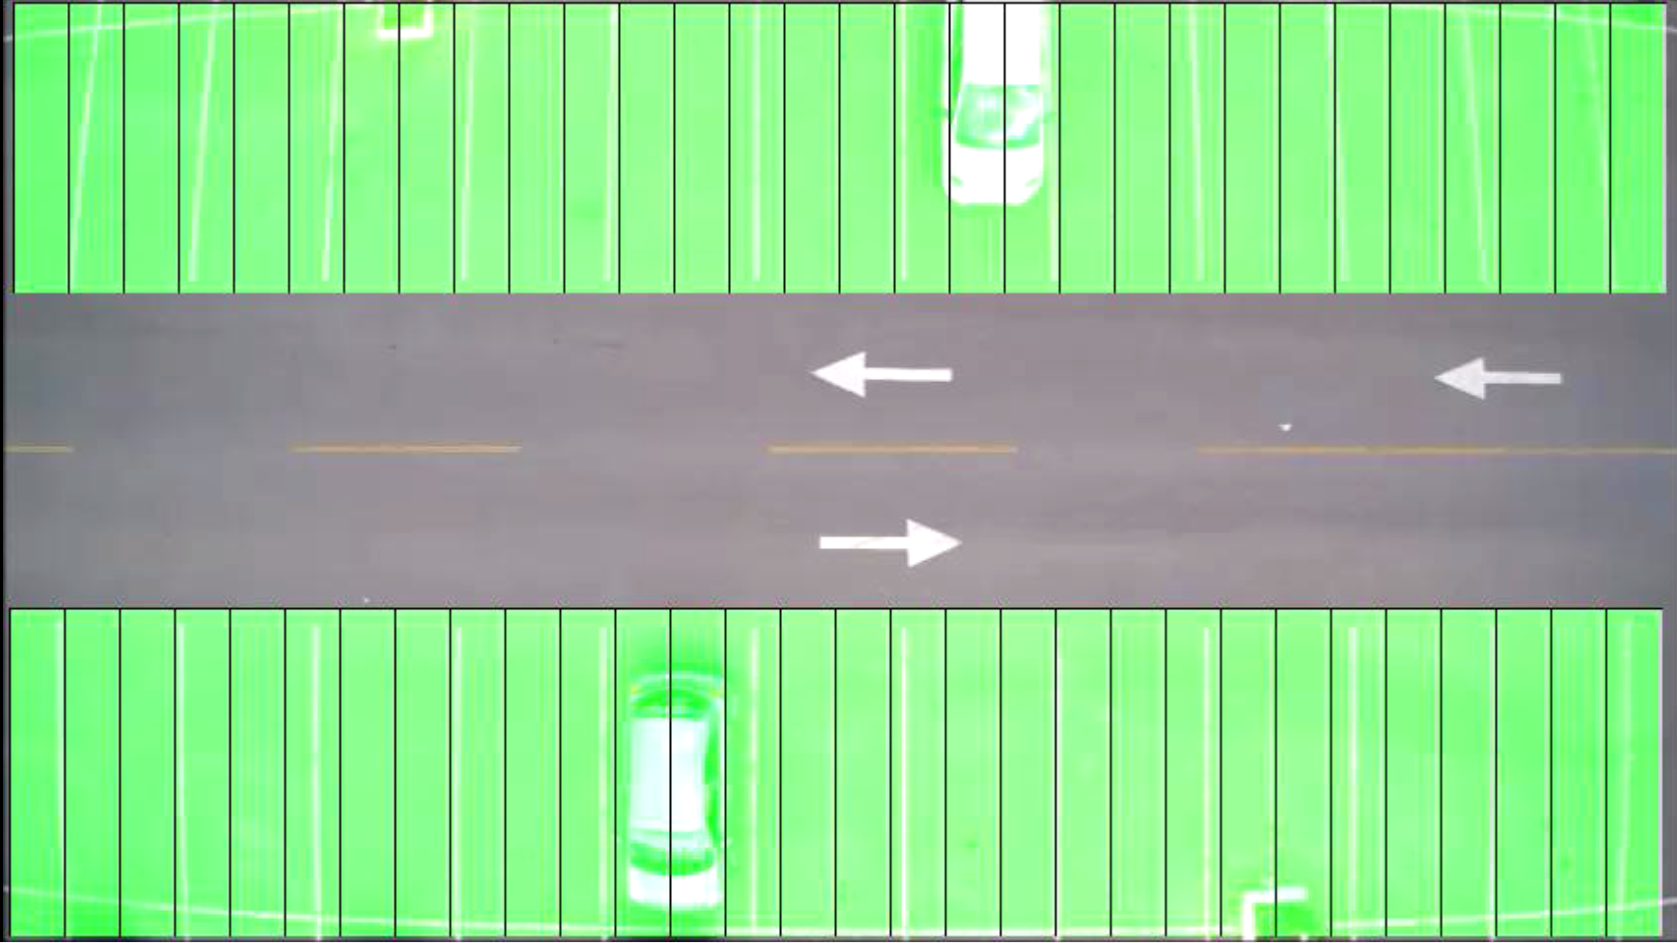
\includegraphics[width=.8\linewidth]{Video6Inicio}
\caption{}
\end{subfigure}\
\begin{subfigure}{.5\textwidth}
\centering
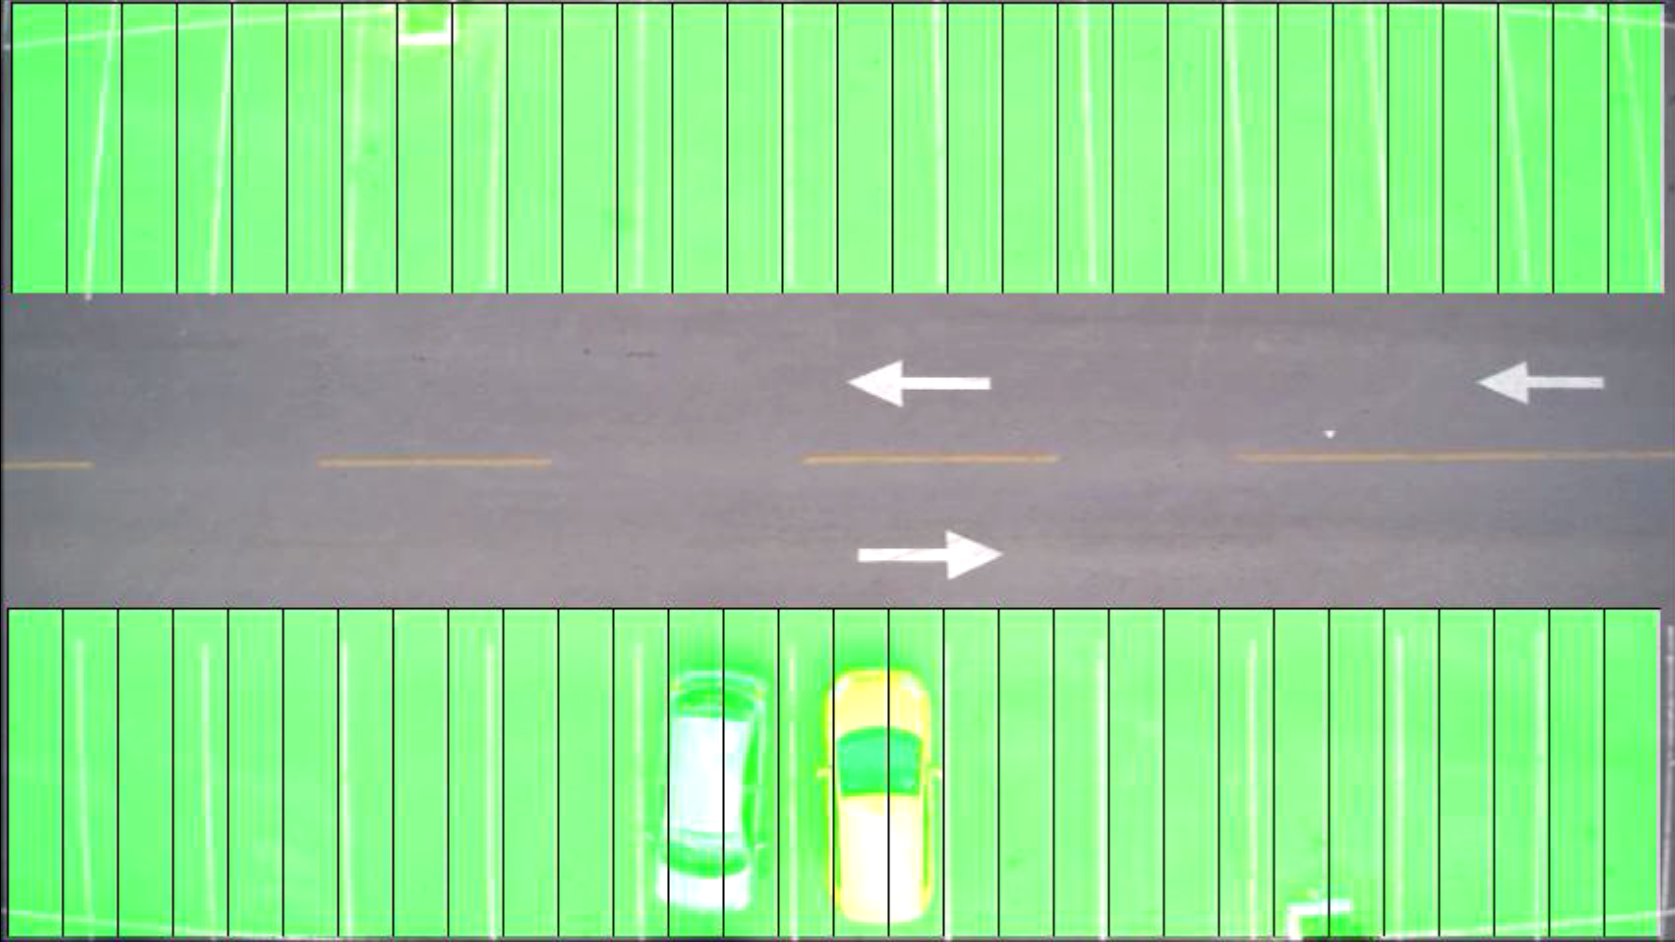
\includegraphics[width=.8\linewidth]{Video6Fim}
\caption{}
\end{subfigure}
\centering
\caption{(a) O momento inicial do vídeo 6. (b) O momento final do vídeo 6.}%
\label{}%
\end{figure}

\subsection{Vídeo 7}

Neste vídeo um dos carros sai da cena pela esquerda. O vídeo tem $17s$ de duração e portanto $1020$ acertos possíveis.

\begin{figure}[!h]
\centering
\begin{subfigure}{.5\textwidth}
\centering
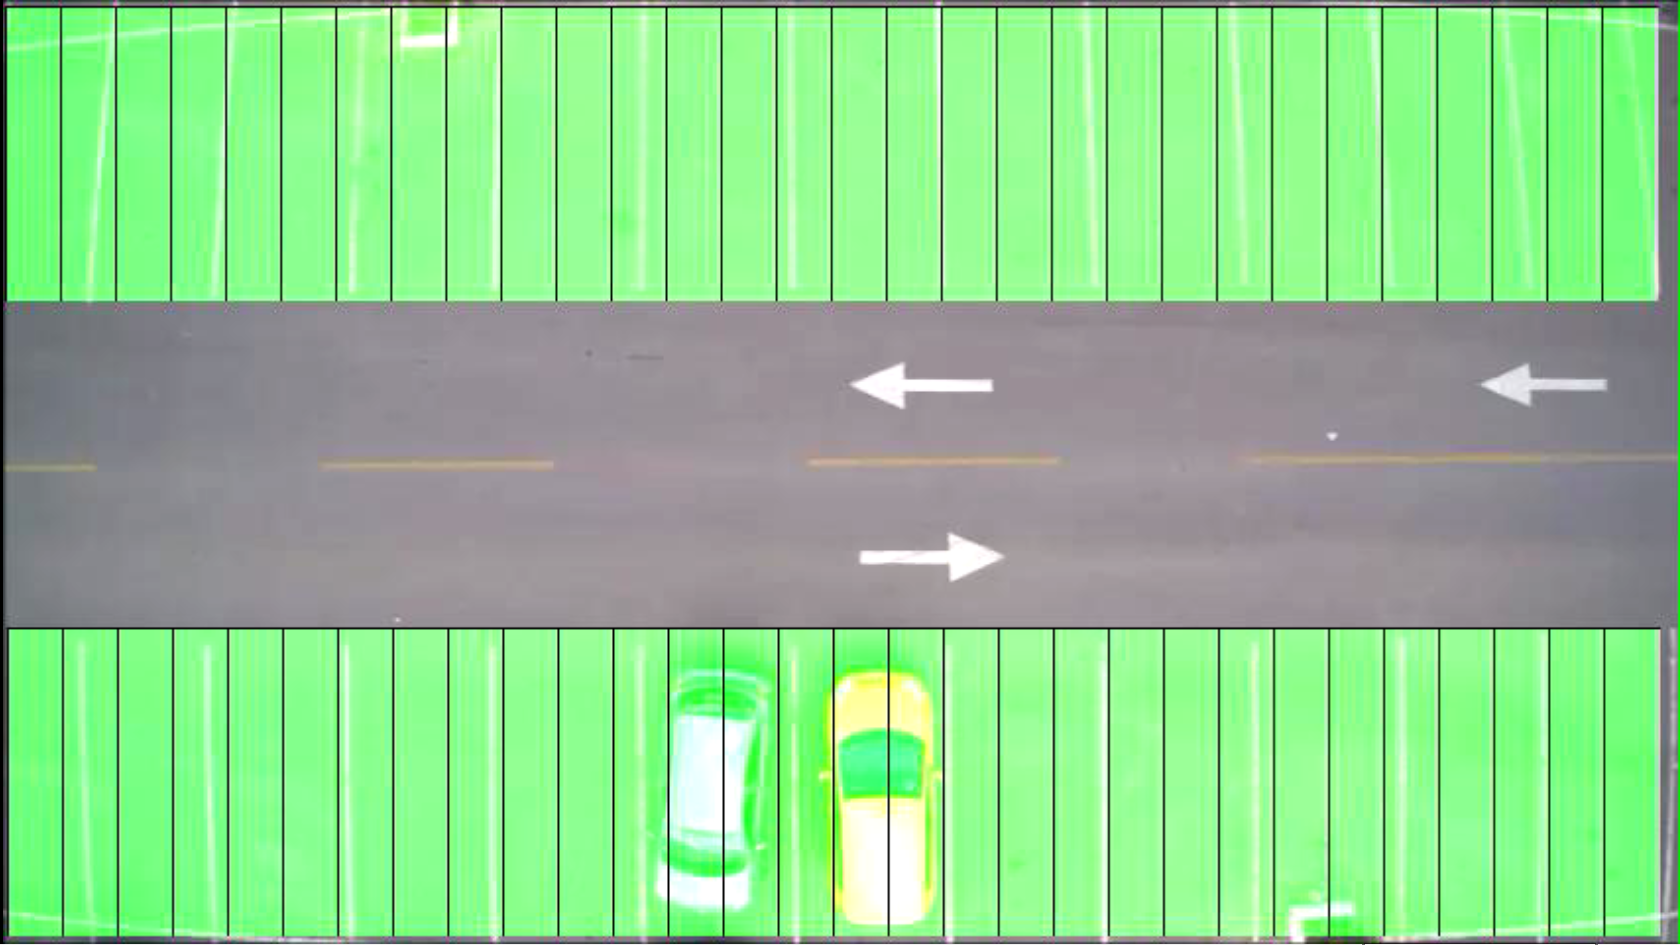
\includegraphics[width=.8\linewidth]{Video7Inicio}
\caption{}
\end{subfigure}\
\begin{subfigure}{.5\textwidth}
\centering
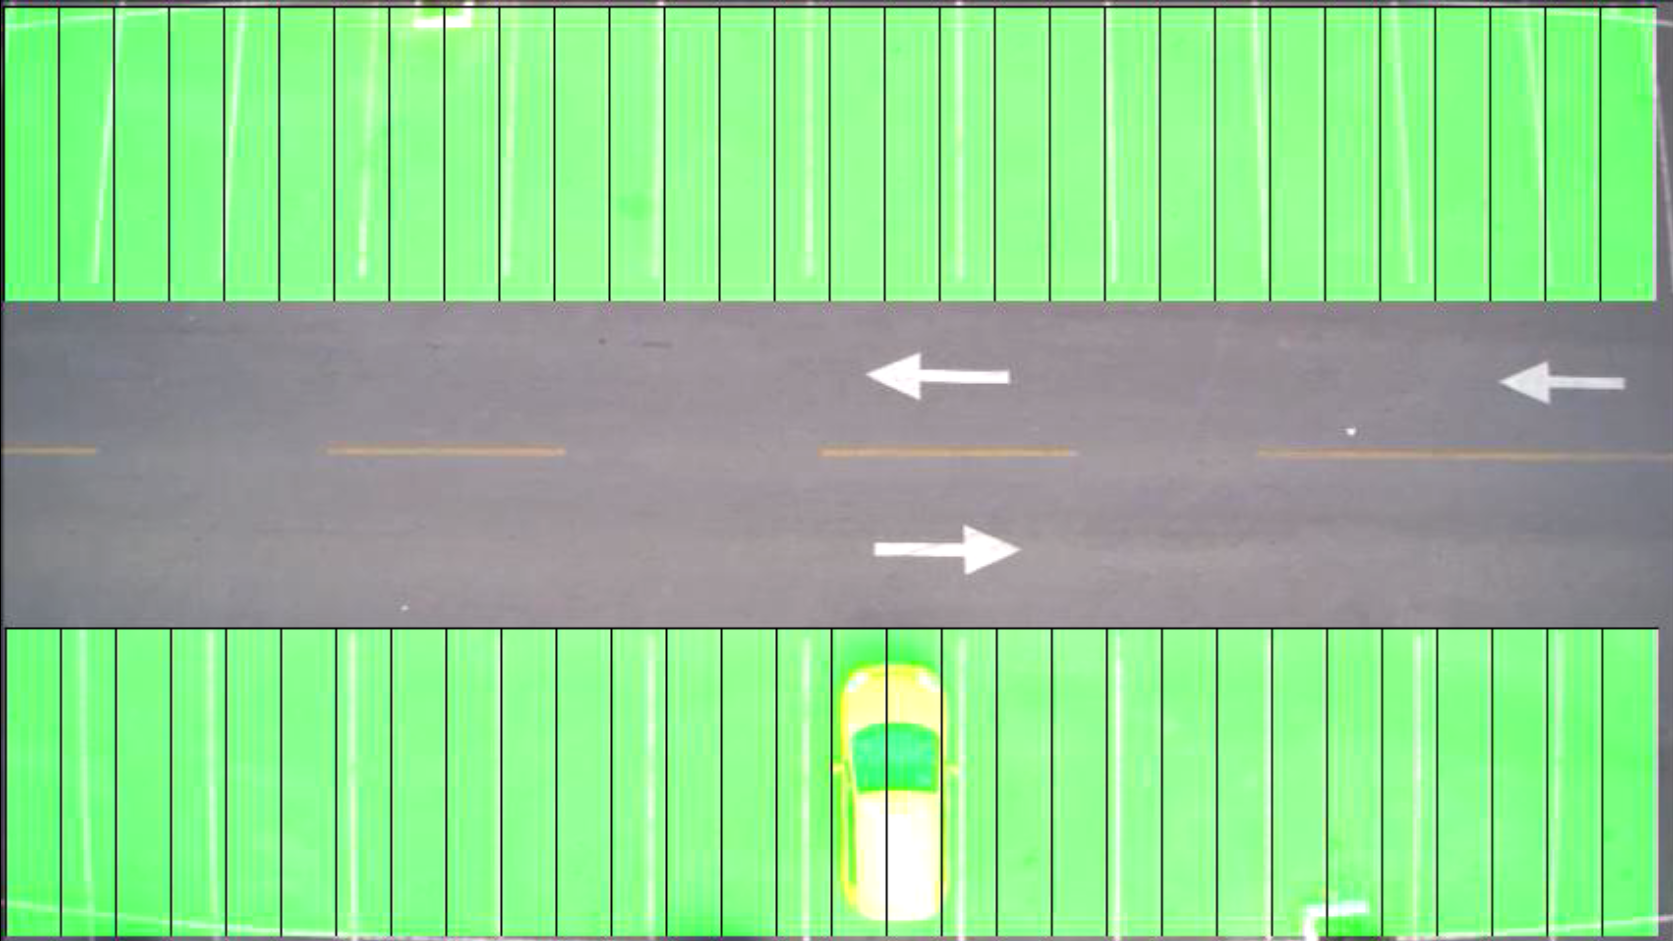
\includegraphics[width=.8\linewidth]{Video7Fim}
\caption{}
\end{subfigure}
\centering
\caption{(a) O momento inicial do vídeo 7. (b) O momento final do vídeo 7.}%
\label{}%
\end{figure}

\subsection{Vídeo 8}

No oitavo e último caso de testes, um carro branco passa pela região central da imagem sem estacionar em nenhuma vaga e depois um carro cinza estaciona na região inferior. O vídeo tem $23s$ de duração e $1380$ acertos possíveis.

\begin{figure}[!h]
\centering
\begin{subfigure}{.5\textwidth}
\centering
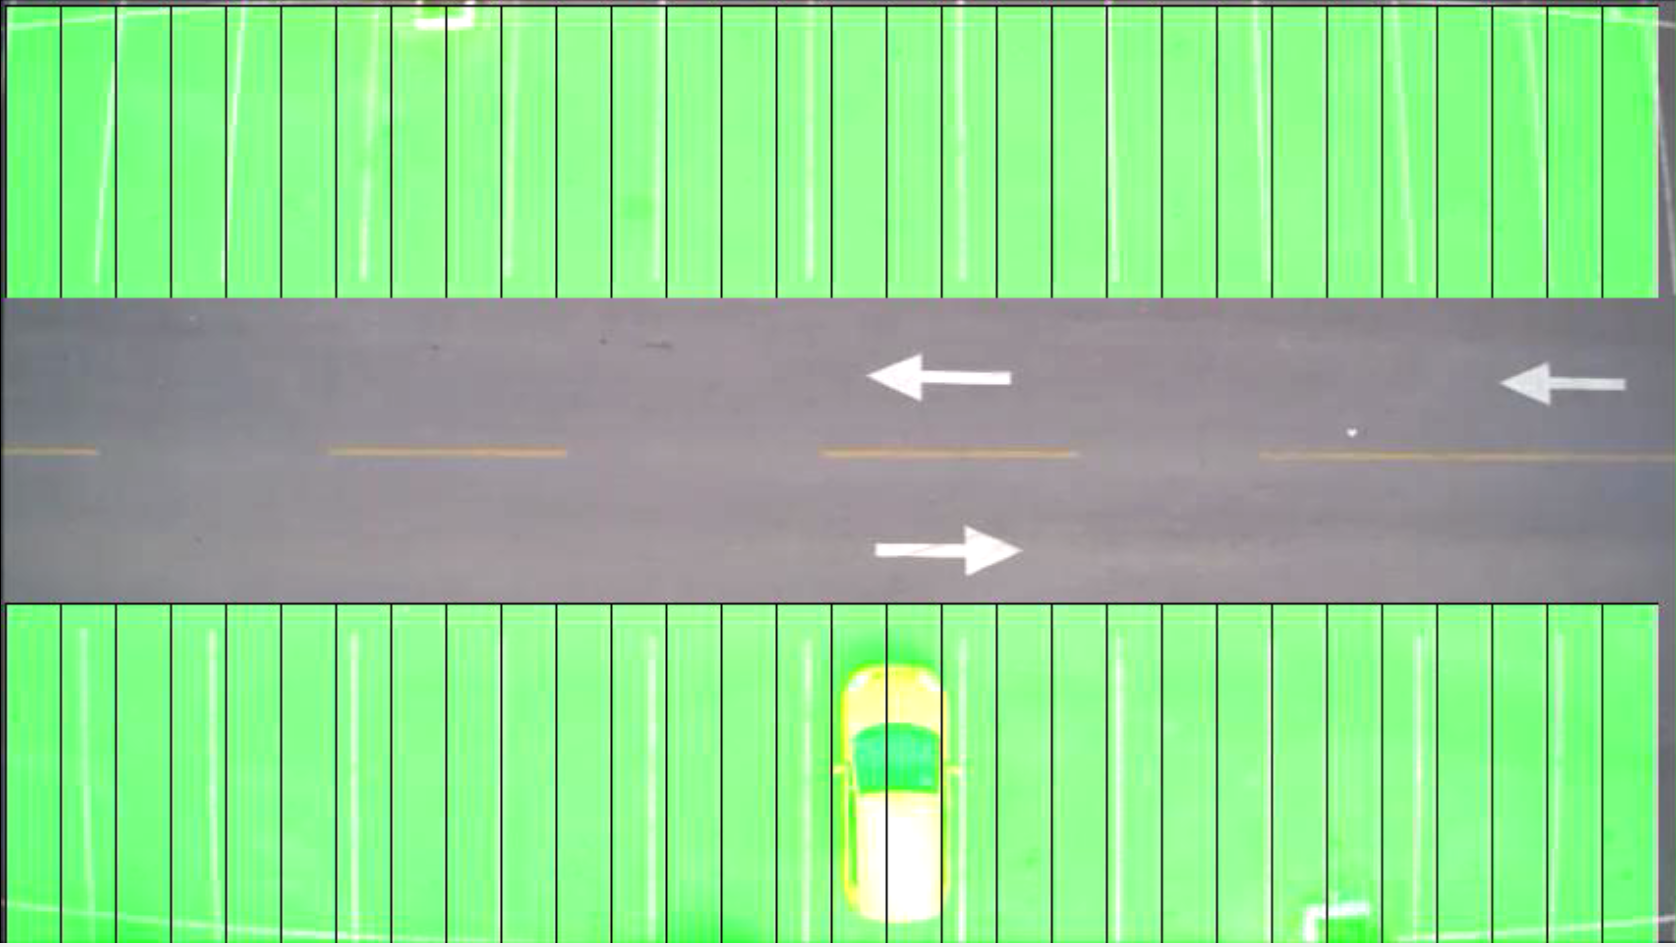
\includegraphics[width=.8\linewidth]{Video8Inicio}
\caption{}
\end{subfigure}\
\begin{subfigure}{.5\textwidth}
\centering
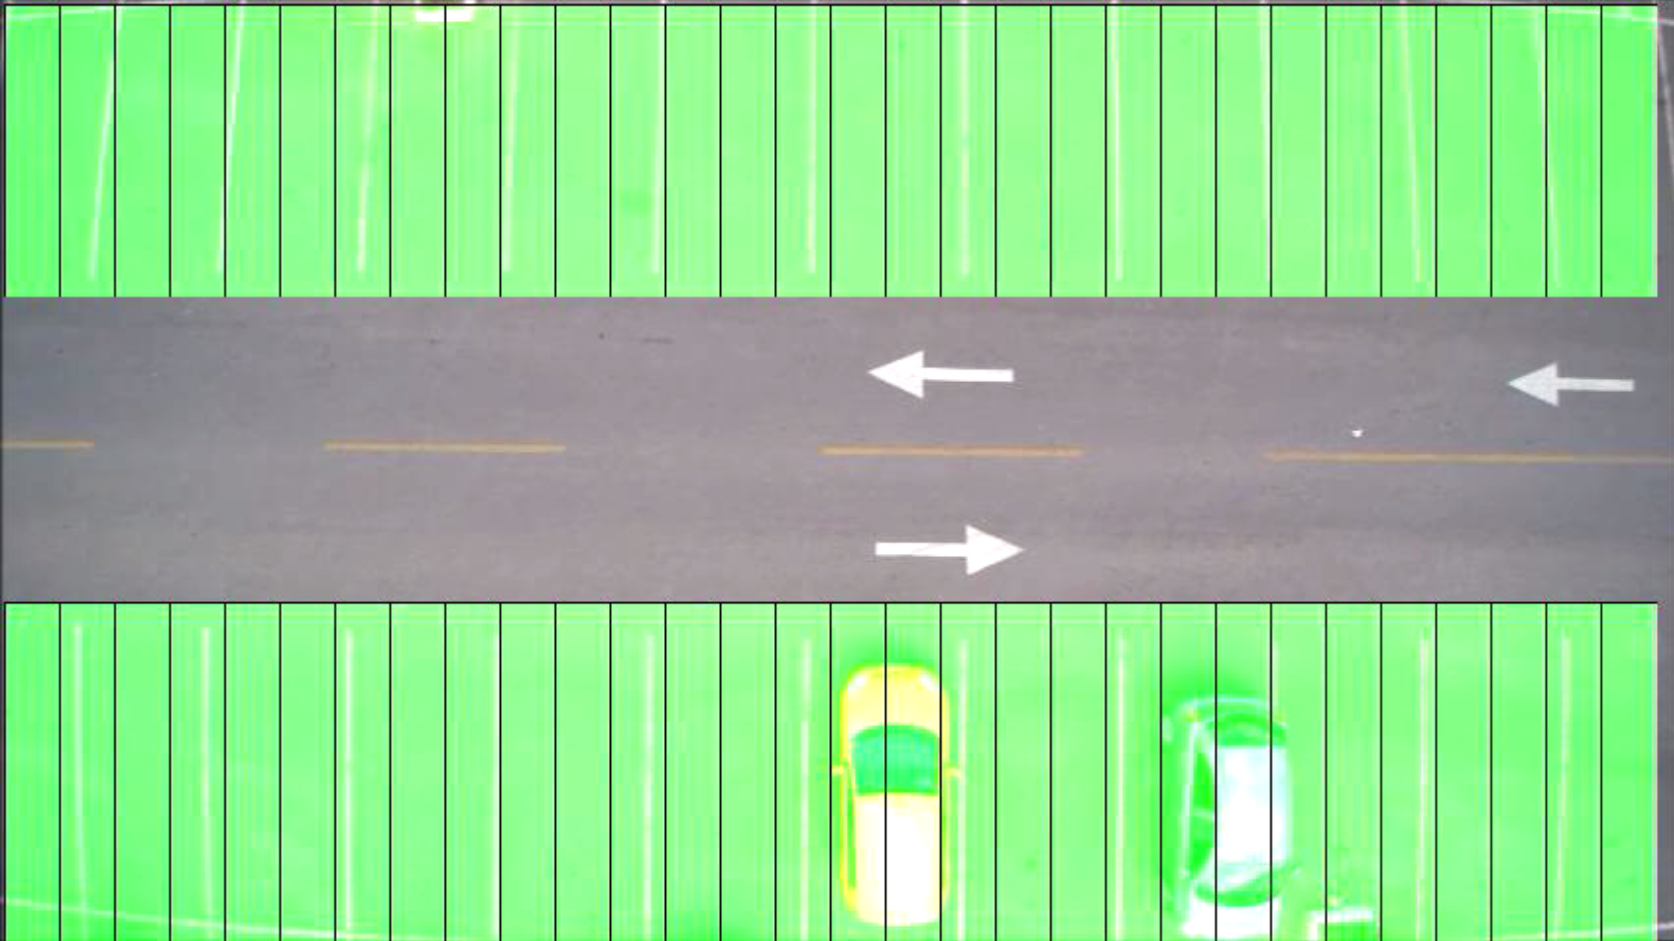
\includegraphics[width=.8\linewidth]{Video8Fim}
\caption{}
\end{subfigure}
\centering
\caption{(a) O momento inicial do vídeo 8. (b) O momento final do vídeo 8.}%
\label{}%
\end{figure}














